% ============================================================
% Synchronous generator operating modes
% Content file for the Power System Simulation with LTspice book.
% All formatting is provided by the central preamble.tex.
% ============================================================

\chapter{Operating Modes of Synchronous Generators}
\label{chap:synchronous-generator-operating-modes}
\index{synchronous generator!operating modes}
\index{synchronous generator!island operation}
\index{synchronous generator!grid-connected operation}
\index{synchronous generator!constant-speed operation}

This chapter demonstrates three important operating modes of a synchronous
generator:

\begin{itemize}
  \item isolated or island operation,
  \item operation connected to a stiff power network, and
  \item operation at fixed mechanical speed.
\end{itemize}

The examples illustrate voltage and speed control, synchronization, active-
and reactive-power control, load-angle stability, and the behaviour of the
machine during symmetrical and asymmetrical faults.

% ============================================================
\section{Isolated Operation}
\label{sec:sg-isolated-operation}
% ============================================================

\subsection{General}

In isolated operation, no external voltage source maintains the network
voltage or frequency. An automatic voltage regulator (AVR) is therefore
required to regulate the terminal voltage, while a speed governor must balance
the mechanical input power against the electrical load. The example also
demonstrates how a second synchronous generator can be synchronized with the
island network.

Adding generators can increase the total inertia and improve the response of
the island system. Stable load sharing, however, requires suitable governor
and excitation-control characteristics.

\begin{important}{Control requirements in island operation}{imp:island-control}
An island network requires at least one unit that regulates frequency and at
least one unit that regulates voltage. In practical parallel operation,
governor droop and AVR reactive-power or voltage droop are normally used to
share active and reactive power between the generators.
\end{important}

\subsection{Circuit Design}

The circuit \texttt{Simulation\_Start} contains a round-rotor synchronous generator rated at
\SI{400}{\mega\watt} and \SI{20}{\kilo\volt}. It is connected through a
transformer rated at \SI{20}{\kilo\volt} on the generator side and
\SI{400}{\kilo\volt} on the network side. A switch connects the generator
to the initially unloaded network at \SI{1}{\second}.
The load increases linearly from zero to \SI{50}{\mega\watt} between
\SI{2}{\second} and \SI{5}{\second}. The AVR is enabled at
\SI{6}{\second}, whereas the speed governor remains active throughout the
simulation. During the first second, the main field winding is supplied by a
temporary excitation ramp from \SI{600}{\volt} to \SI{1400}{\volt} and
back to \SI{600}{\volt}. This accelerates the buildup of the rated terminal
voltage.
The AVR measures the voltage on the high-voltage side and uses a reference of
\SI{400}{\kilo\volt}. The governor reference is
\SI{1500}{\rpm}. Its switching time is placed outside the simulated interval,
for example at \SI{500}{\second}, so that the controller remains active.
Both external controllers are implemented as simple PI controllers to
illustrate the fundamental behaviour of the controlled machine. Their dynamics
are intentionally fast in order to shorten the simulation.

\begin{simulation}{AVR switching sequence}{sim:island-avr-switching}
The AVR switch must close shortly before the switch supplying the fixed field
voltage opens. The field voltage must not be interrupted, because this would
cause the terminal voltage to collapse. Since the excitation circuit may carry
a high current, the switch on-resistance must be sufficiently small to avoid an
unwanted field-voltage drop.

The torque-control changeover is less critical. Owing to the large moment of
inertia $J$, the rotor speed cannot change abruptly even if the electromagnetic
or mechanical torque is briefly disturbed.
\end{simulation}

\subsection{Simulation Start} see Figures: \ref{fig:figure81} and \ref{fig:figure82}  (simulation-file: same name as the heading)

The machine starts with zero terminal voltage. The initial field-voltage boost
to \SI{1400}{\volt} allows the rated voltage to be reached quickly. For this
demonstration, the stator copper-resistance parameter \texttt{Rcu} is set to
\num{0.01} to accelerate voltage buildup and thereby reduce simulation time.

\subsection{Voltage Behaviour} see Figures: \ref{fig:figure81} and \ref{fig:figure82}

After approximately \SI{1}{\second}, the network voltage reaches
\SI{400}{\kilo\volt}, corresponding to \SI{20}{\kilo\volt} at the
generator terminals. As the load rises from zero to
\SI{50}{\mega\watt}, the network voltage falls slightly to approximately
\SI{397}{\kilo\volt}. When the AVR is enabled at \SI{6}{\second}, it
rapidly restores the voltage to \SI{400}{\kilo\volt}.

In an island network, a voltage change can also change the active and reactive
power absorbed by voltage-dependent loads. For an ideal constant-power load,
by contrast, the specified active and reactive powers remain constant and the
current changes as the voltage changes.

\subsection{Speed Behaviour} see Figures: \ref{fig:figure81} and \ref{fig:figure82}

During the load ramp, the speed initially falls below \SI{1500}{\rpm}. Once
the final load has been reached and the governor has increased the mechanical
torque, the speed returns to its reference value. When the AVR is enabled, the
rising voltage temporarily increases the load current and electromagnetic
torque. Consequently, the frequency briefly decreases before returning to its
steady-state value.

\subsection{Load Angle and Load Steps} see Figures: \ref{fig:figure83}-\ref{fig:figure86}  (simulation-file: same names as the heading)

During the first load ramp, the load angle increases and settles at
approximately \ang{12}. A \SI{30}{\mega\watt} load step can be introduced
by setting \texttt{Vfact=3} at \SI{2}{\second} and closing an additional
switch at \SI{3}{\second}. Further load steps at \SI{5}{\second} and
\SI{7}{\second} increase the generator output from
\SI{30}{\mega\watt} to \SI{60}{\mega\watt} and finally to
\SI{90}{\mega\watt}. The maximum load angle is approximately \ang{21}.

Each load step produces a transient change in frequency and load angle. The
governor subsequently establishes a new torque balance.

\begin{figure}[H]
	\centering
	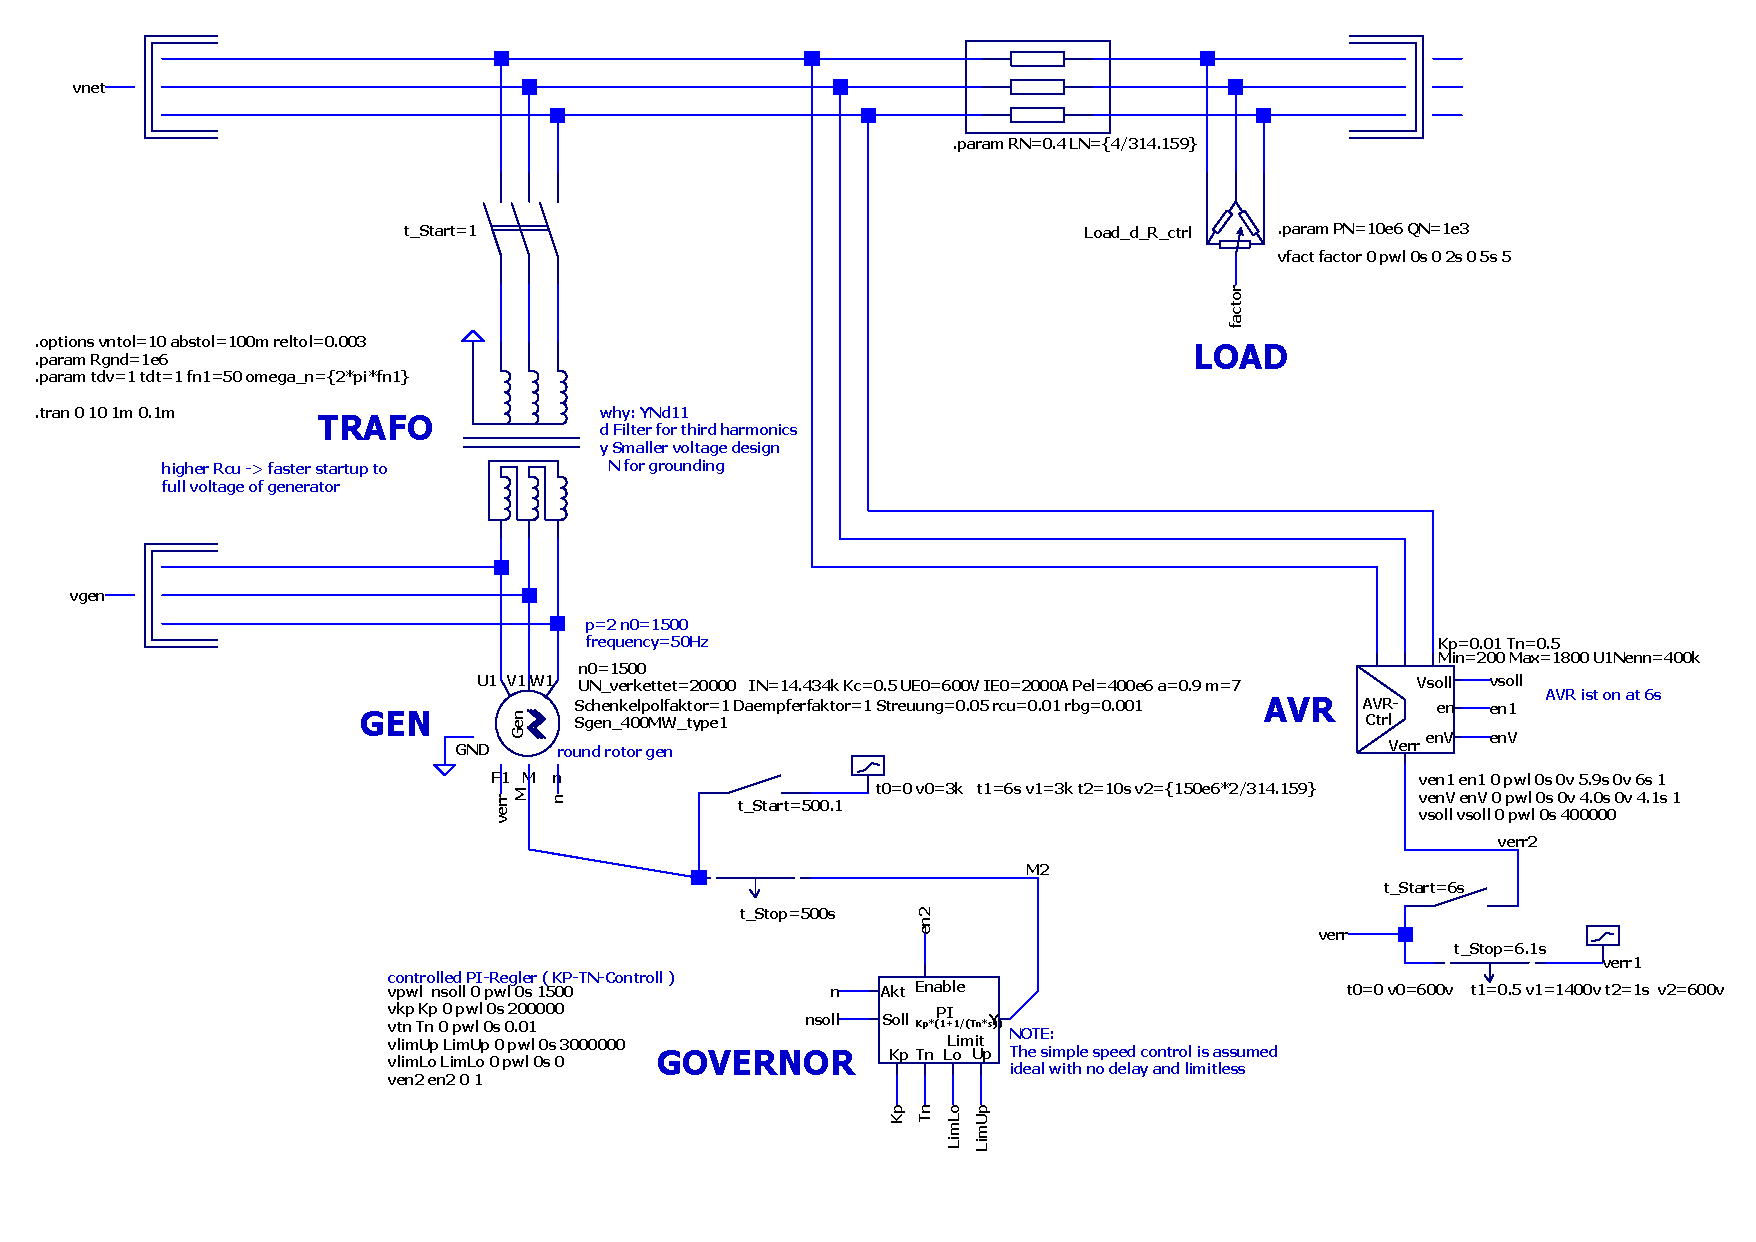
\includegraphics[width=1\textwidth] {figures/08_Synchronous_Generator/Synchronous_Generator_Isolated_mode_500MVA/Simulation_Start_Schematic.pdf}
	\caption{Simulation start - Voltage behaviour - Speed behaviour  - schematic}
	\label{fig:figure81}
\end{figure}

\begin{figure}[H]
	\centering
	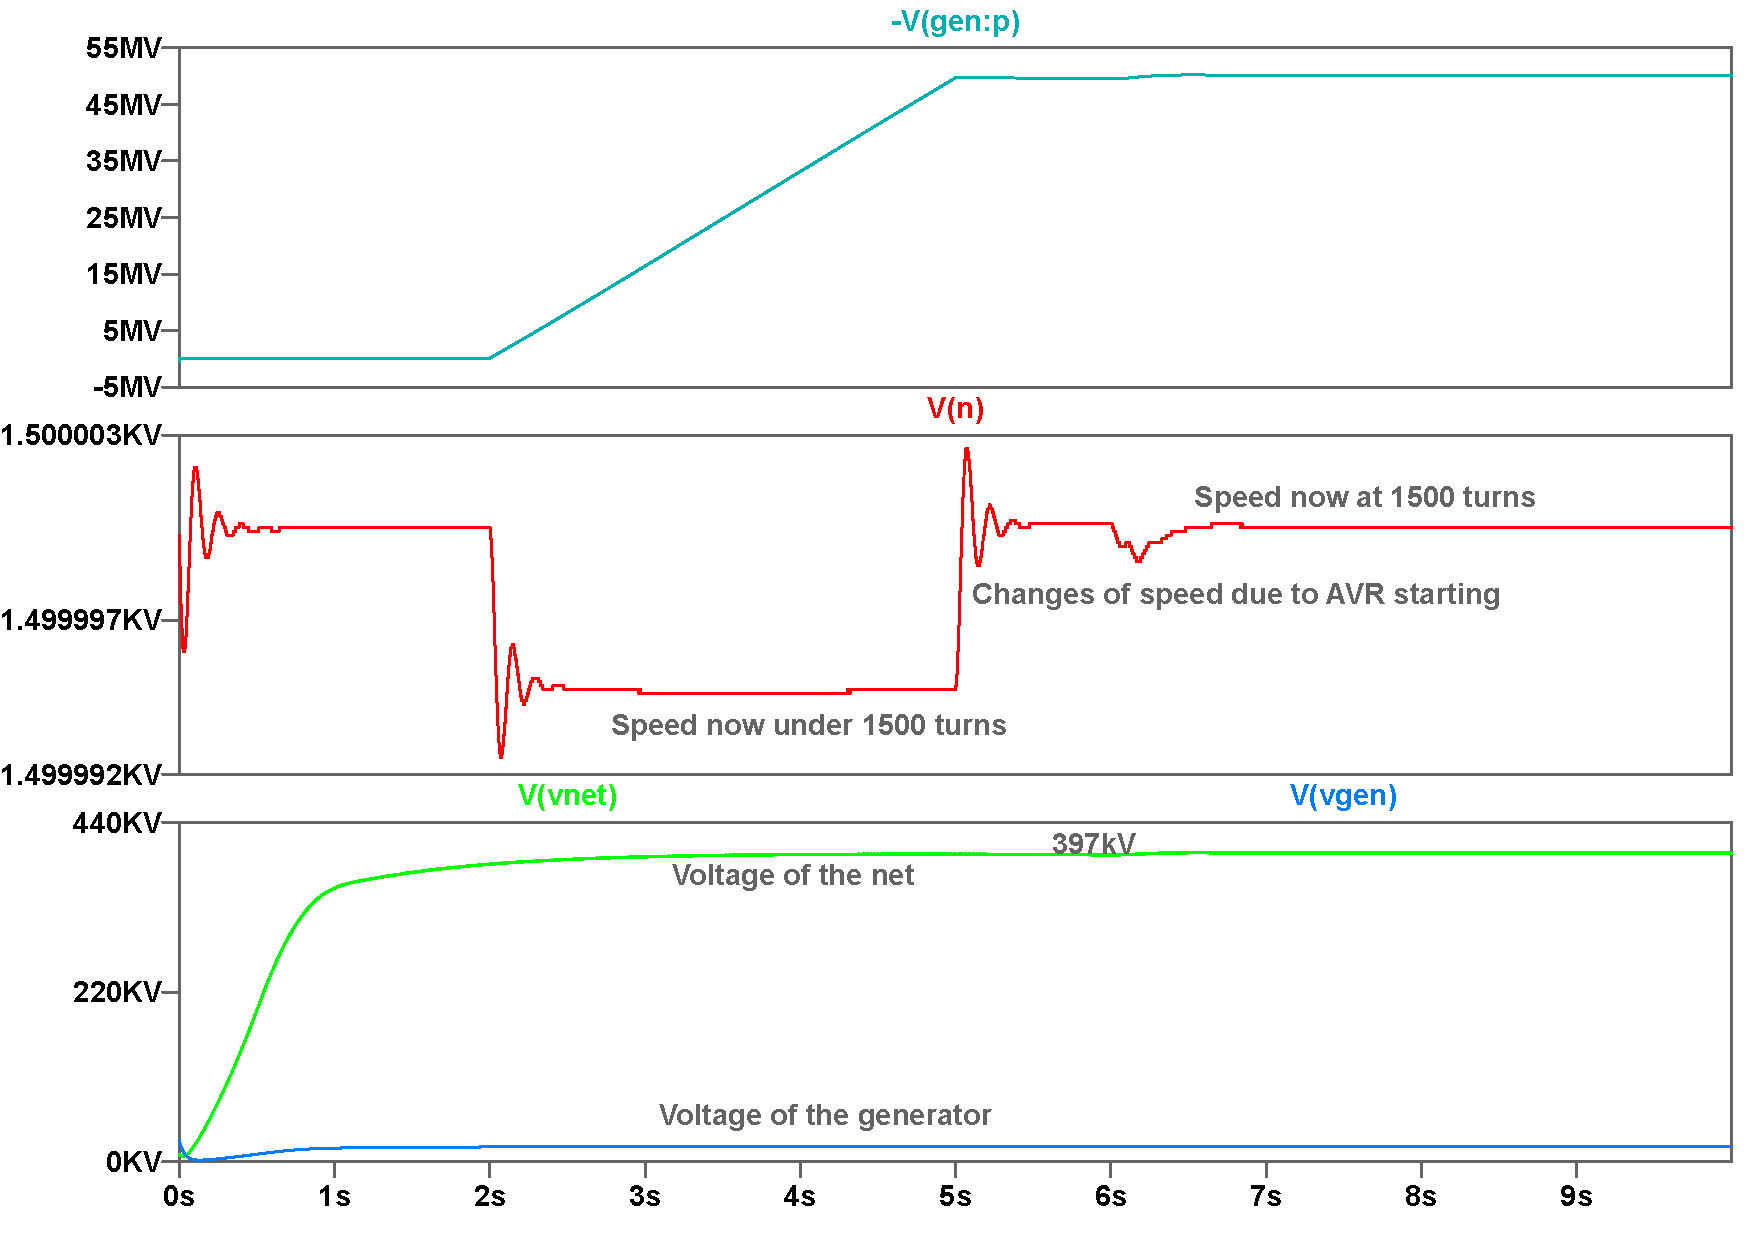
\includegraphics[width=0.9\textwidth] {figures/08_Synchronous_Generator/Synchronous_Generator_Isolated_mode_500MVA/Simulation_Start_Waveform.pdf}
	\caption{Simulaton start - Voltage behaviour - Speed behaviour - Waveform}
	\label{fig:figure82}
\end{figure}

\begin{figure}[H]
	\centering
	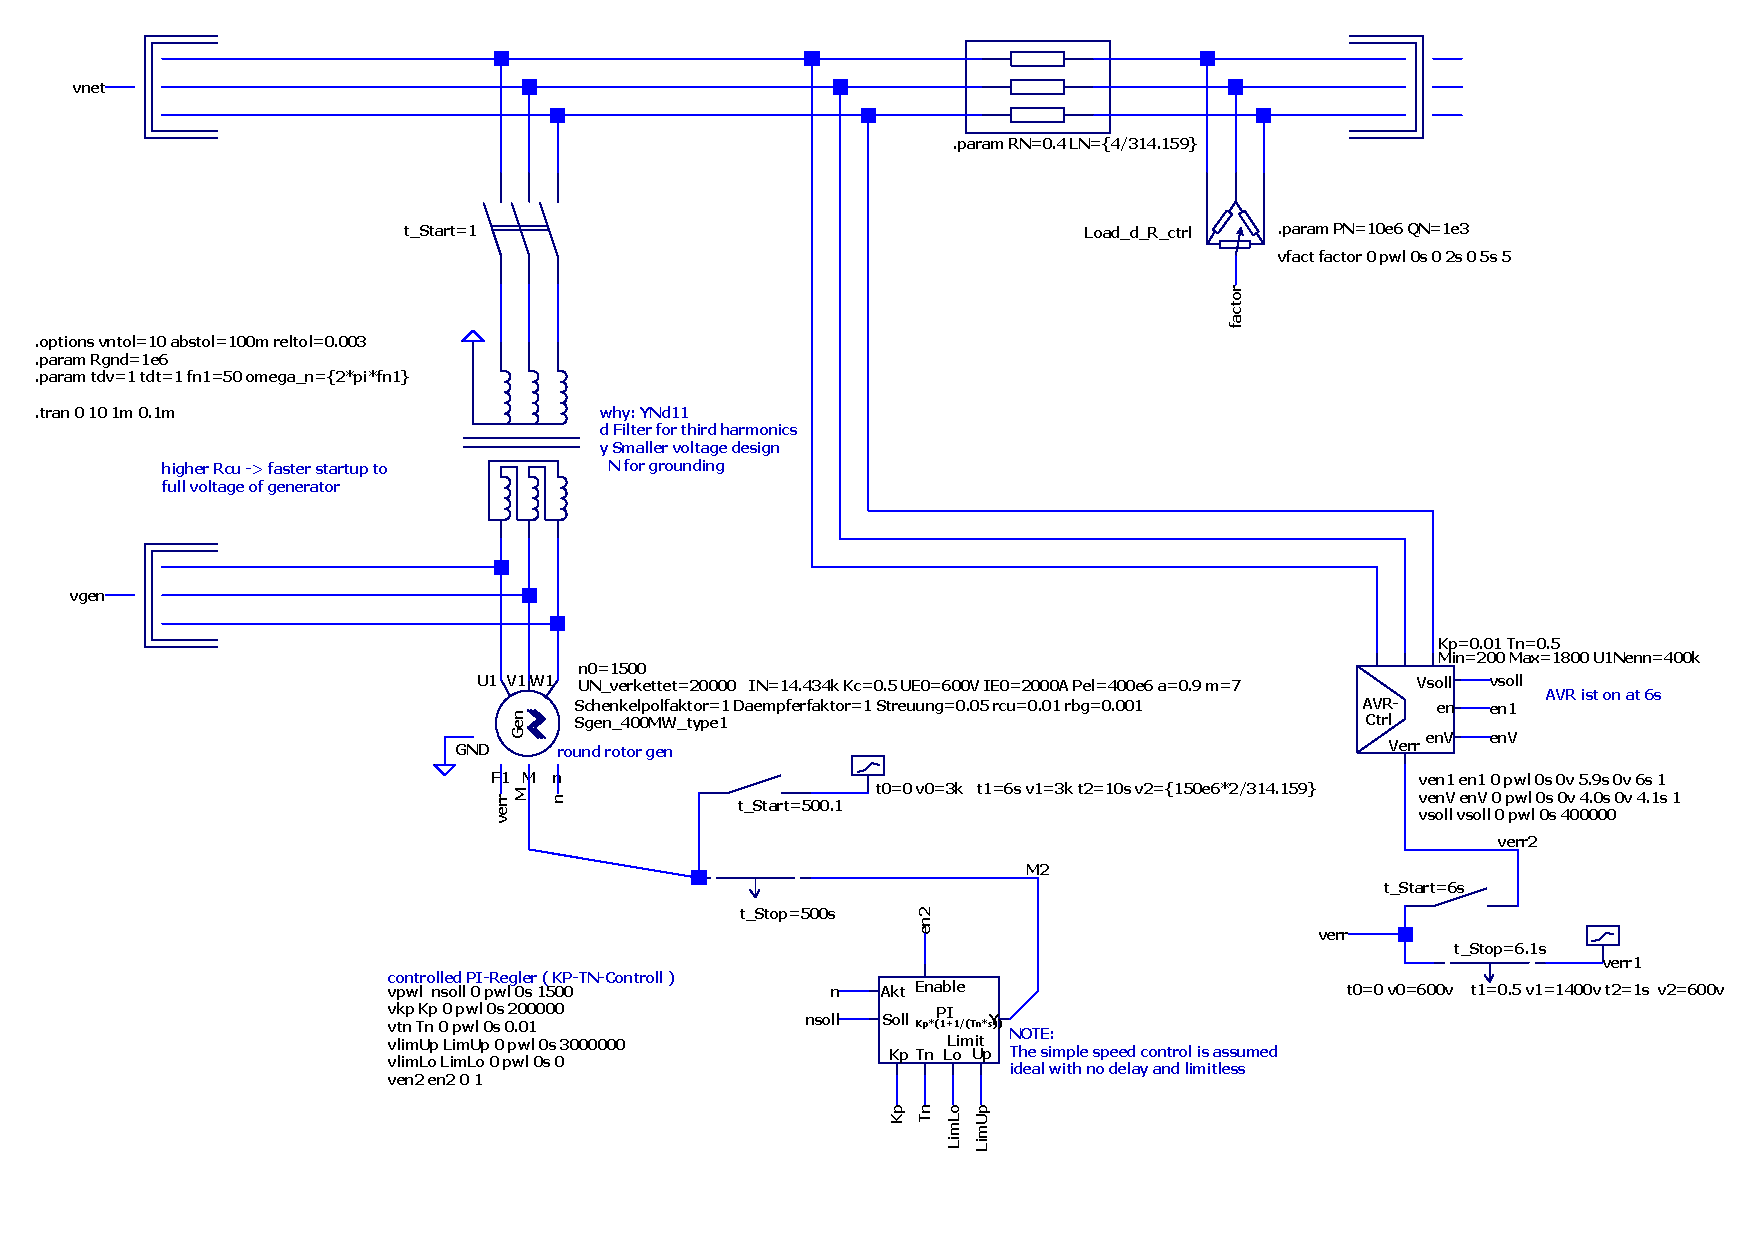
\includegraphics[width=1\textwidth] {figures/08_Synchronous_Generator/Synchronous_Generator_Isolated_mode_500MVA/Load_angle_Schematic.pdf}
	\caption{Load angle - schematic}
	\label{fig:figure83}
\end{figure}

\begin{figure}[H]
	\centering
	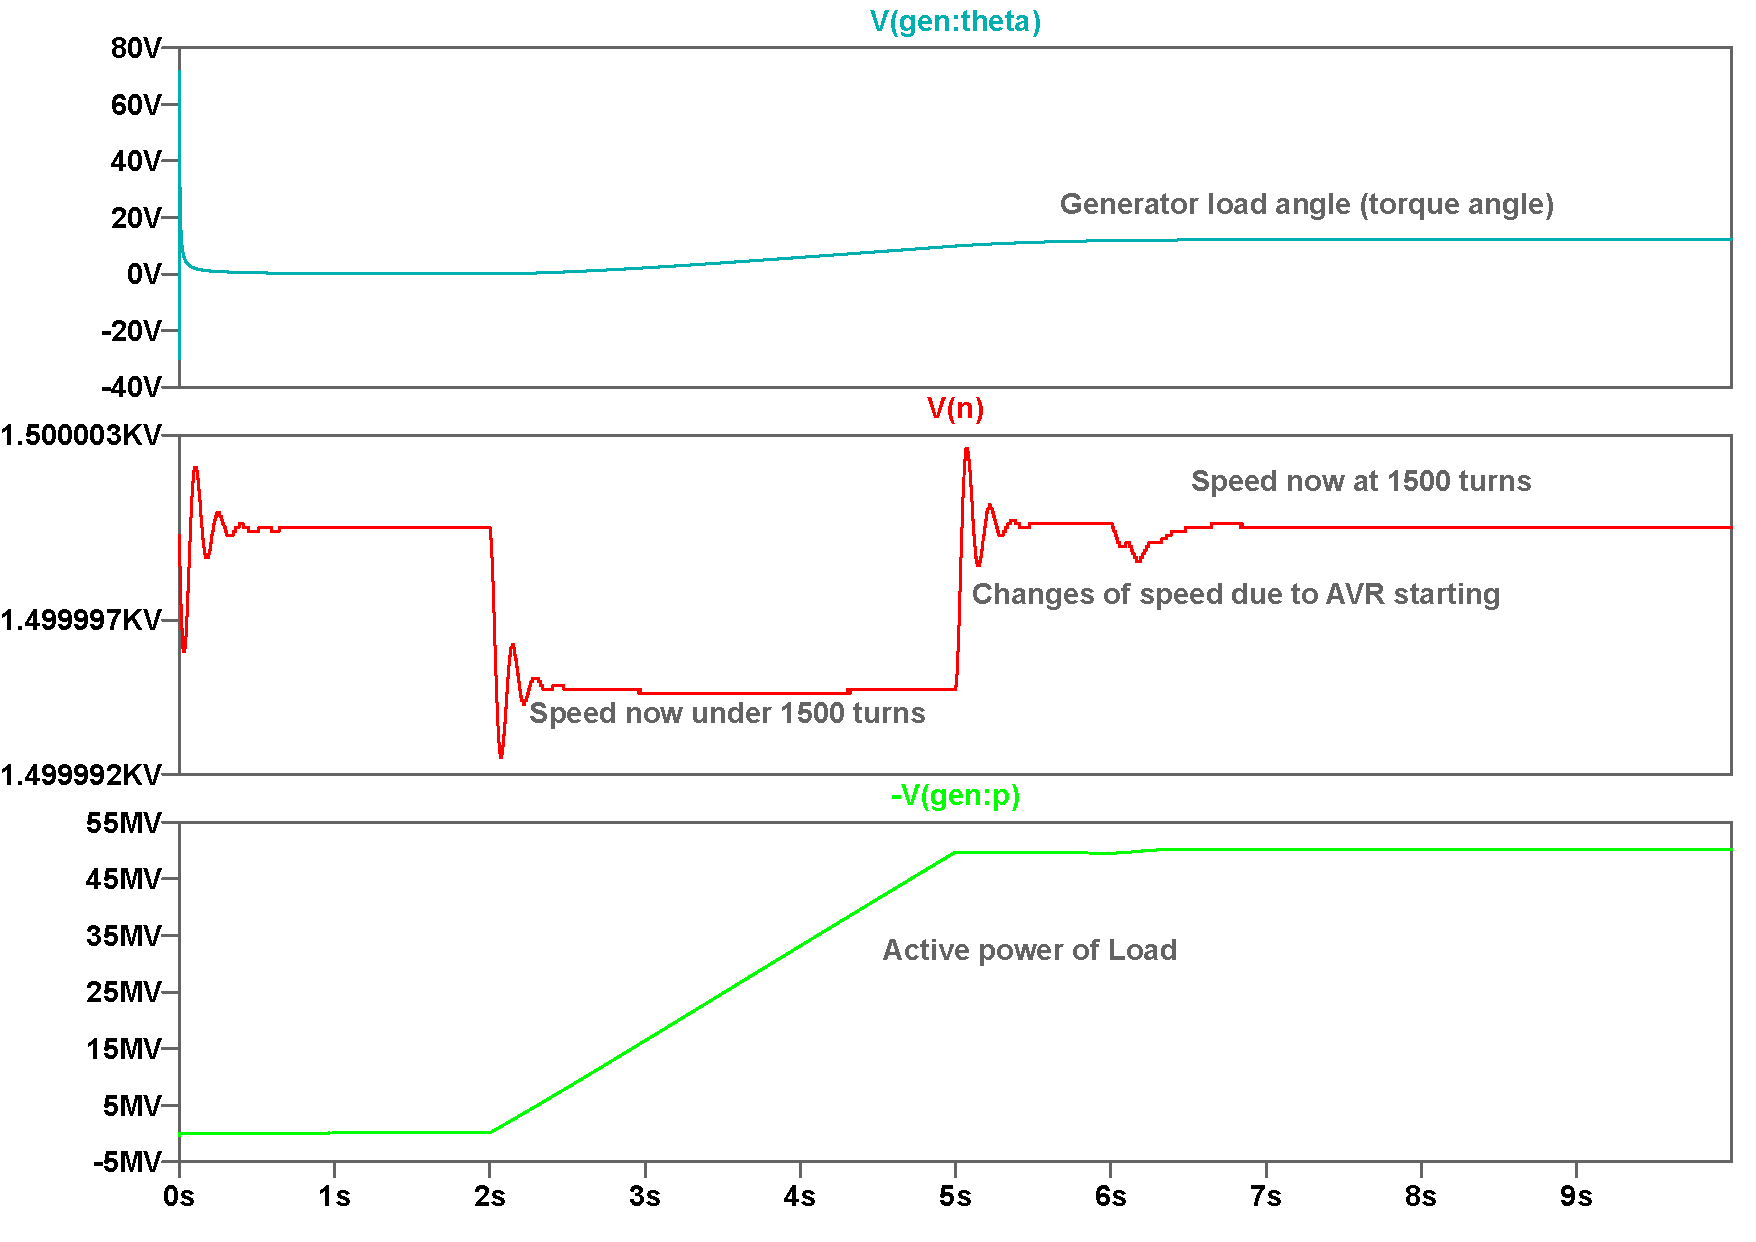
\includegraphics[width=0.9\textwidth] {figures/08_Synchronous_Generator/Synchronous_Generator_Isolated_mode_500MVA/Load_angle_Waveform.pdf}
	\caption{Load angle - Waveform}
	\label{fig:figure84}
\end{figure}

\begin{figure}[H]
	\centering
	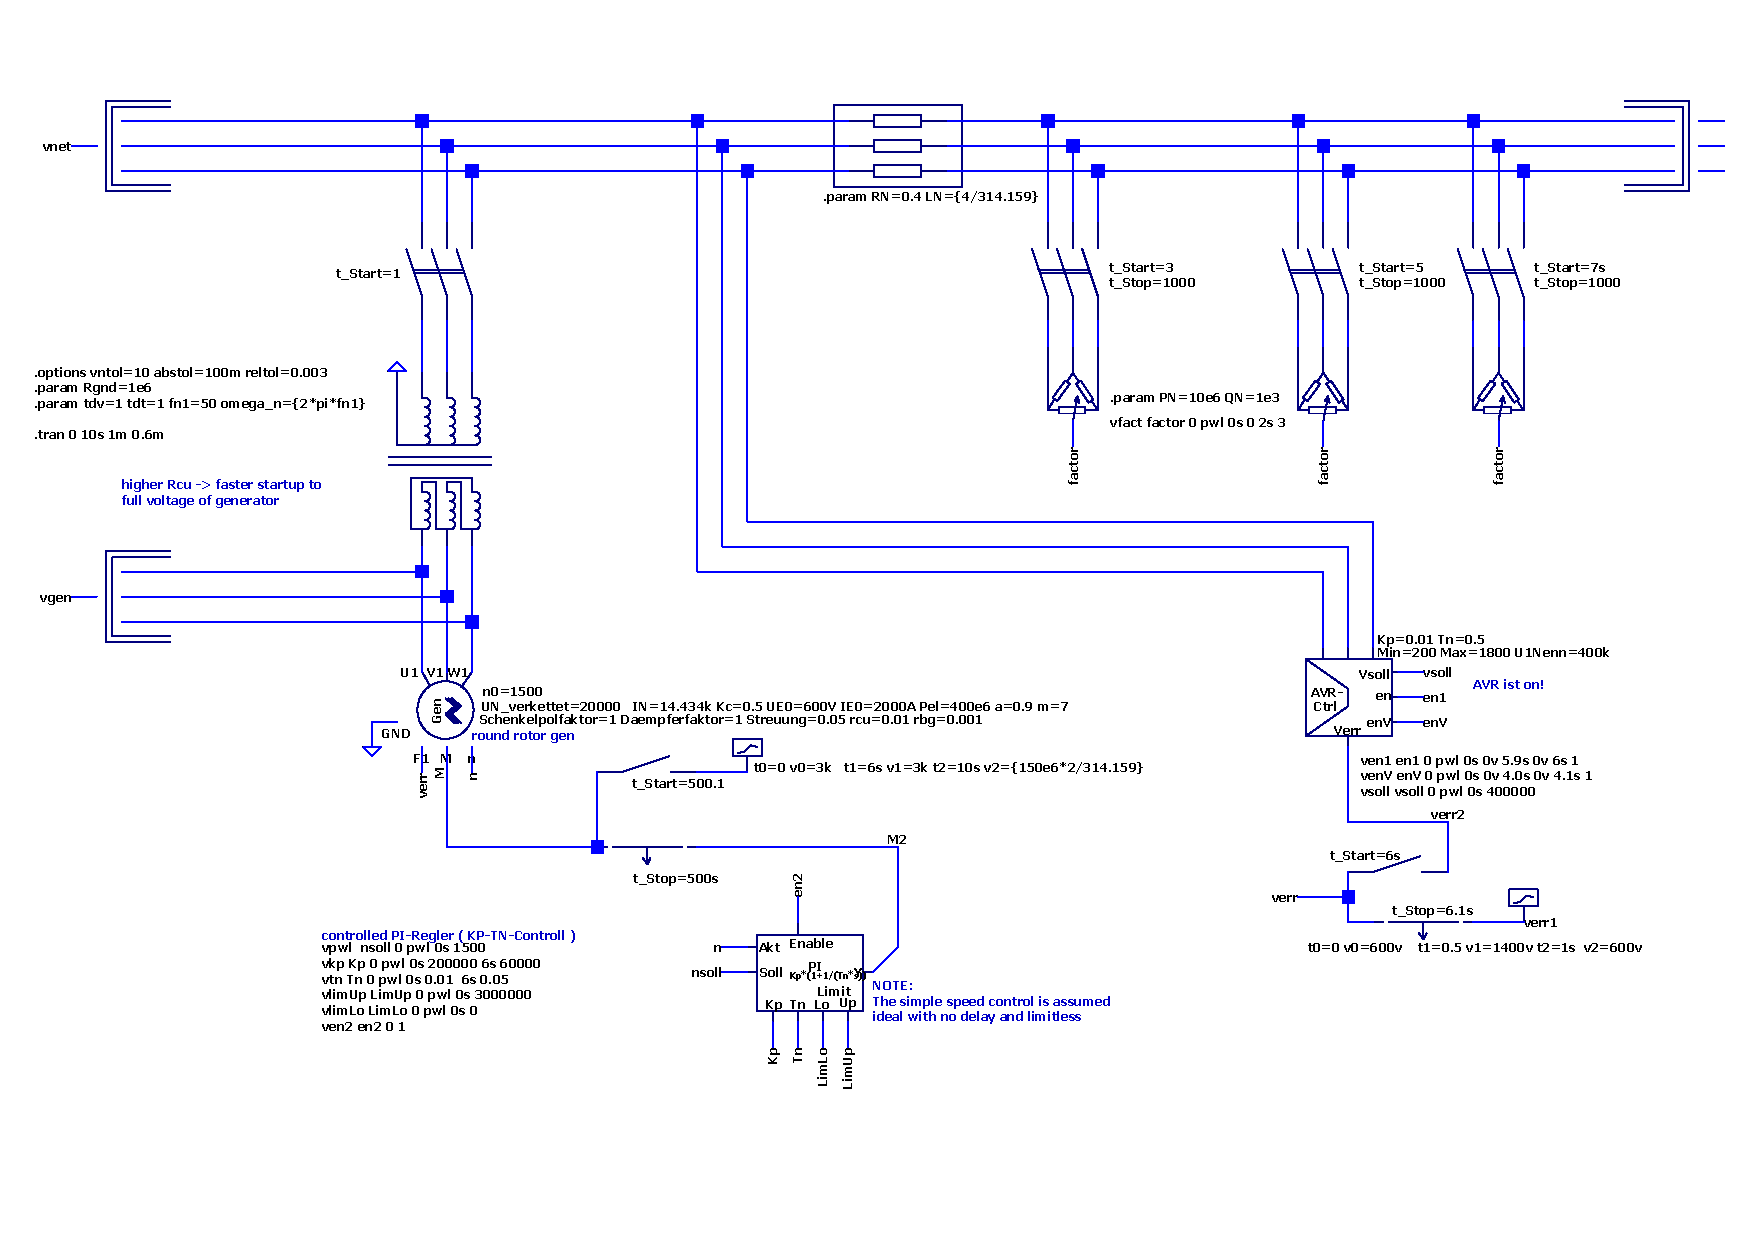
\includegraphics[width=1\textwidth] {figures/08_Synchronous_Generator/Synchronous_Generator_Isolated_mode_500MVA/Load_steps_Schematic.pdf}
	\caption{Load steps - schematic}
	\label{fig:figure85}
\end{figure}

\begin{figure}[H]
	\centering
	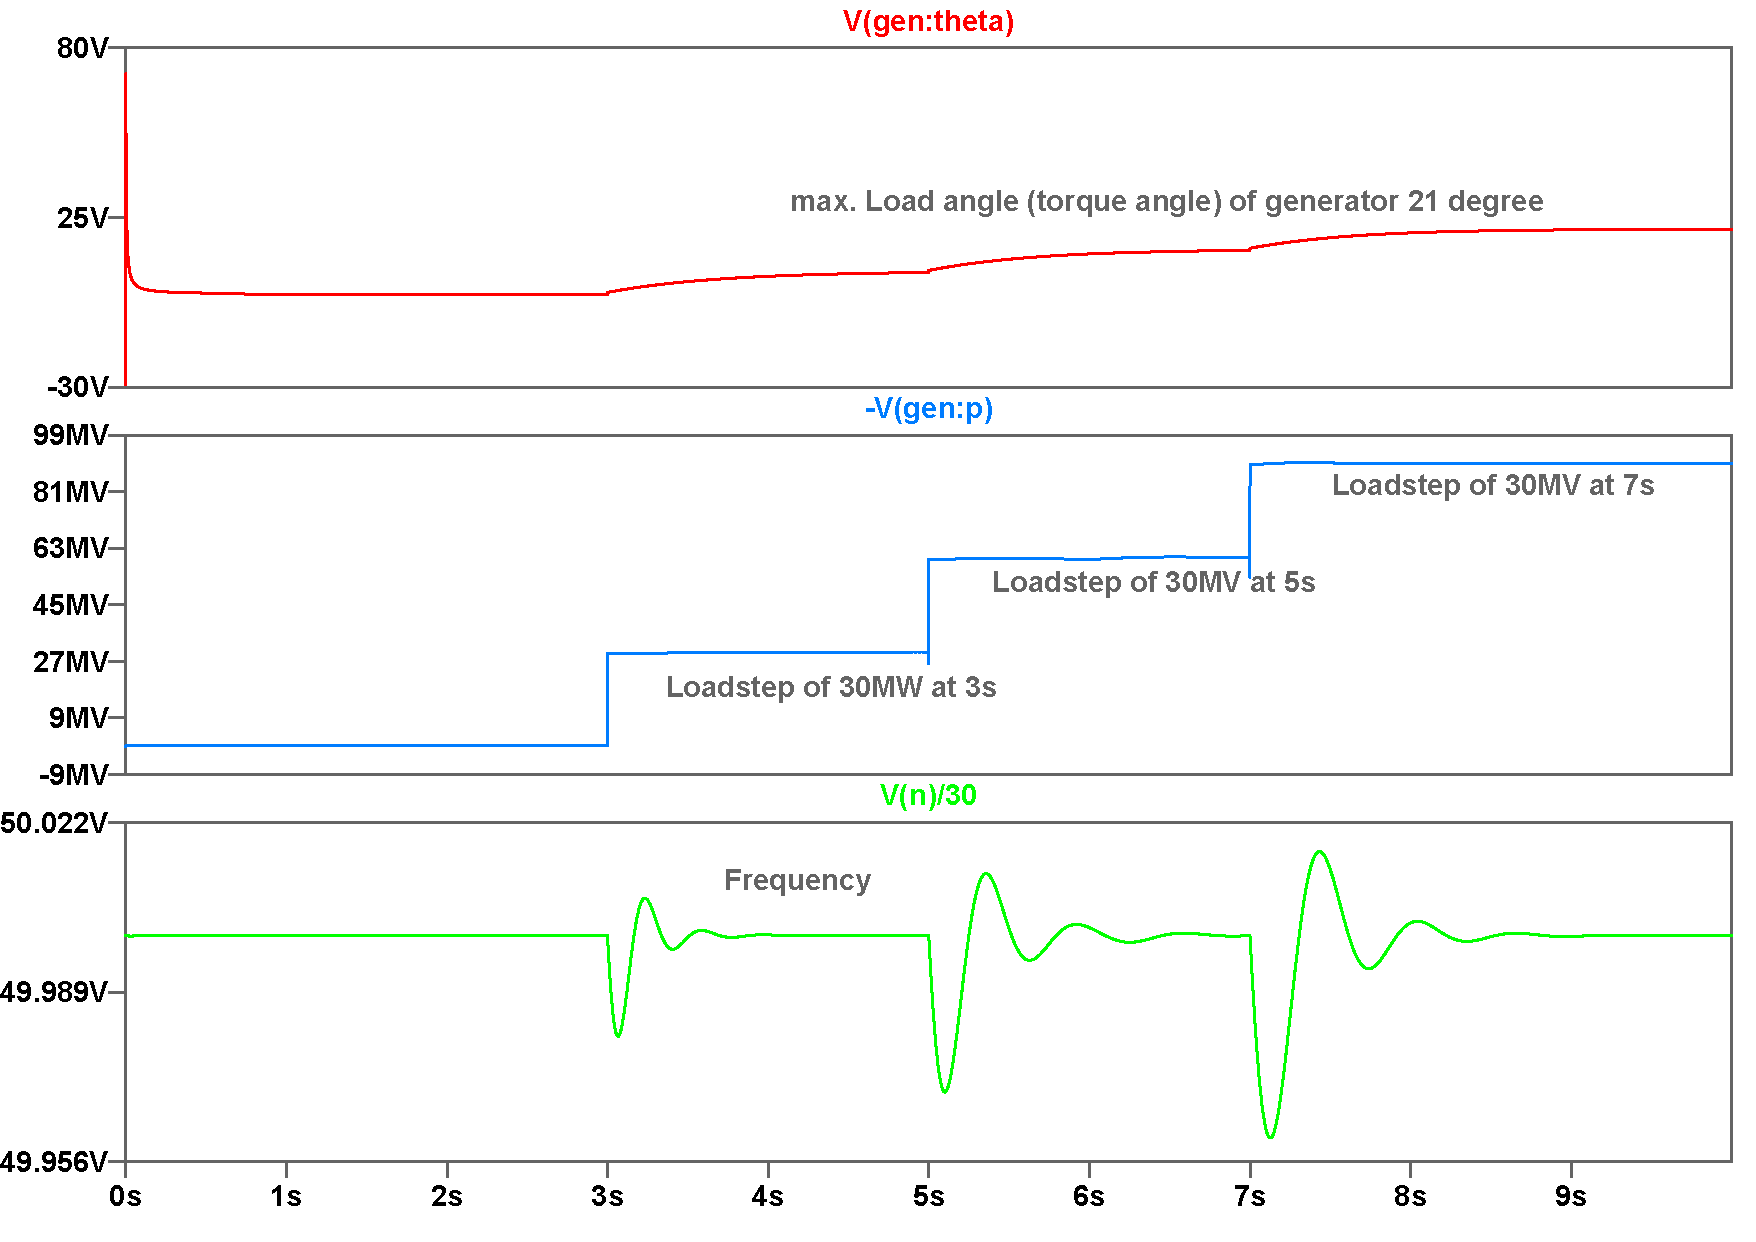
\includegraphics[width=0.9\textwidth] {figures/08_Synchronous_Generator/Synchronous_Generator_Isolated_mode_500MVA/Load_steps_Waveform.pdf}
	\caption{Load steps - Waveform}
	\label{fig:figure86}
\end{figure}


\subsection{Comparison with a Salient-Pole Machine} see figures: \ref{fig:figure87} and \ref{fig:figure88}  (simulation-file: same name as the heading)

The parameter settings \texttt{SchenkelPoleFactor=0.5} and \texttt{KC=0.8}
represent a salient-pole machine in this model. After restarting the
simulation, the load angle is approximately \ang{7}, compared with about
\ang{21} for the round-rotor case. The difference results from the changed
direct- and quadrature-axis reactances and the additional reluctance-torque
component.



\subsection{Reactive Power in Island Operation} 

In an isolated network, the total active and reactive powers are determined by
the connected loads and network losses. Excitation primarily controls the
terminal voltage and the sharing of reactive power between parallel sources.
With only one generator, changing the field voltage cannot independently
specify the reactive power demanded by a constant-power load.

\begin{remark}{Voltage dependence of the load}{rem:island-load-model}
The influence of the AVR on load power depends on the load model. Constant-impedance loads change their power approximately with the square of the
voltage, whereas ideal constant-power loads maintain their specified $P$ and
$Q$ by changing their current.
\end{remark}

\subsection{Switching Off the Loads} see figures: \ref{fig:figure89} and \ref{fig:figure810}  (simulation-file: same name as the heading)

The three loads are disconnected at \SI{9}{\second}, \SI{11}{\second}, and
\SI{13}{\second}. The load angle decreases after each switching operation.
When the final load is removed, the frequency overshoots above its nominal
value, which is the opposite of its response to a positive load step. In the
chosen model, the frequency takes approximately \SI{3.5}{\second} to return
to \SI{50}{\hertz}, because only the governor action and the comparatively
small friction torque decelerate the rotor.

\subsection{Scaling Quantities in the Waveform Viewer} 

Internal signals are always in Volt and can be displayed in engineering units by using the following scale factors in LTspice: e.g 
multiplying a trace for active power (in volt) by 1W/1V gives the
correct unit now in W.

\begin{center}
\renewcommand{\arraystretch}{1.15}
\begin{tabularx}{0.86\textwidth}{@{}l l X@{}}
\toprule
\textbf{Quantity} & \textbf{Scale factor} & \textbf{Displayed unit} \\
\midrule
Load angle & $1\,\mathrm{deg}/\mathrm{V}$ & degree \\
Frequency  & $1\,\mathrm{Hz}/\mathrm{V}$  & hertz \\
Active power & $1\,\mathrm{W}/\mathrm{V}$ & watt \\
\bottomrule
\end{tabularx}
\end{center}

\newpage


\begin{figure}[H]
	\centering
	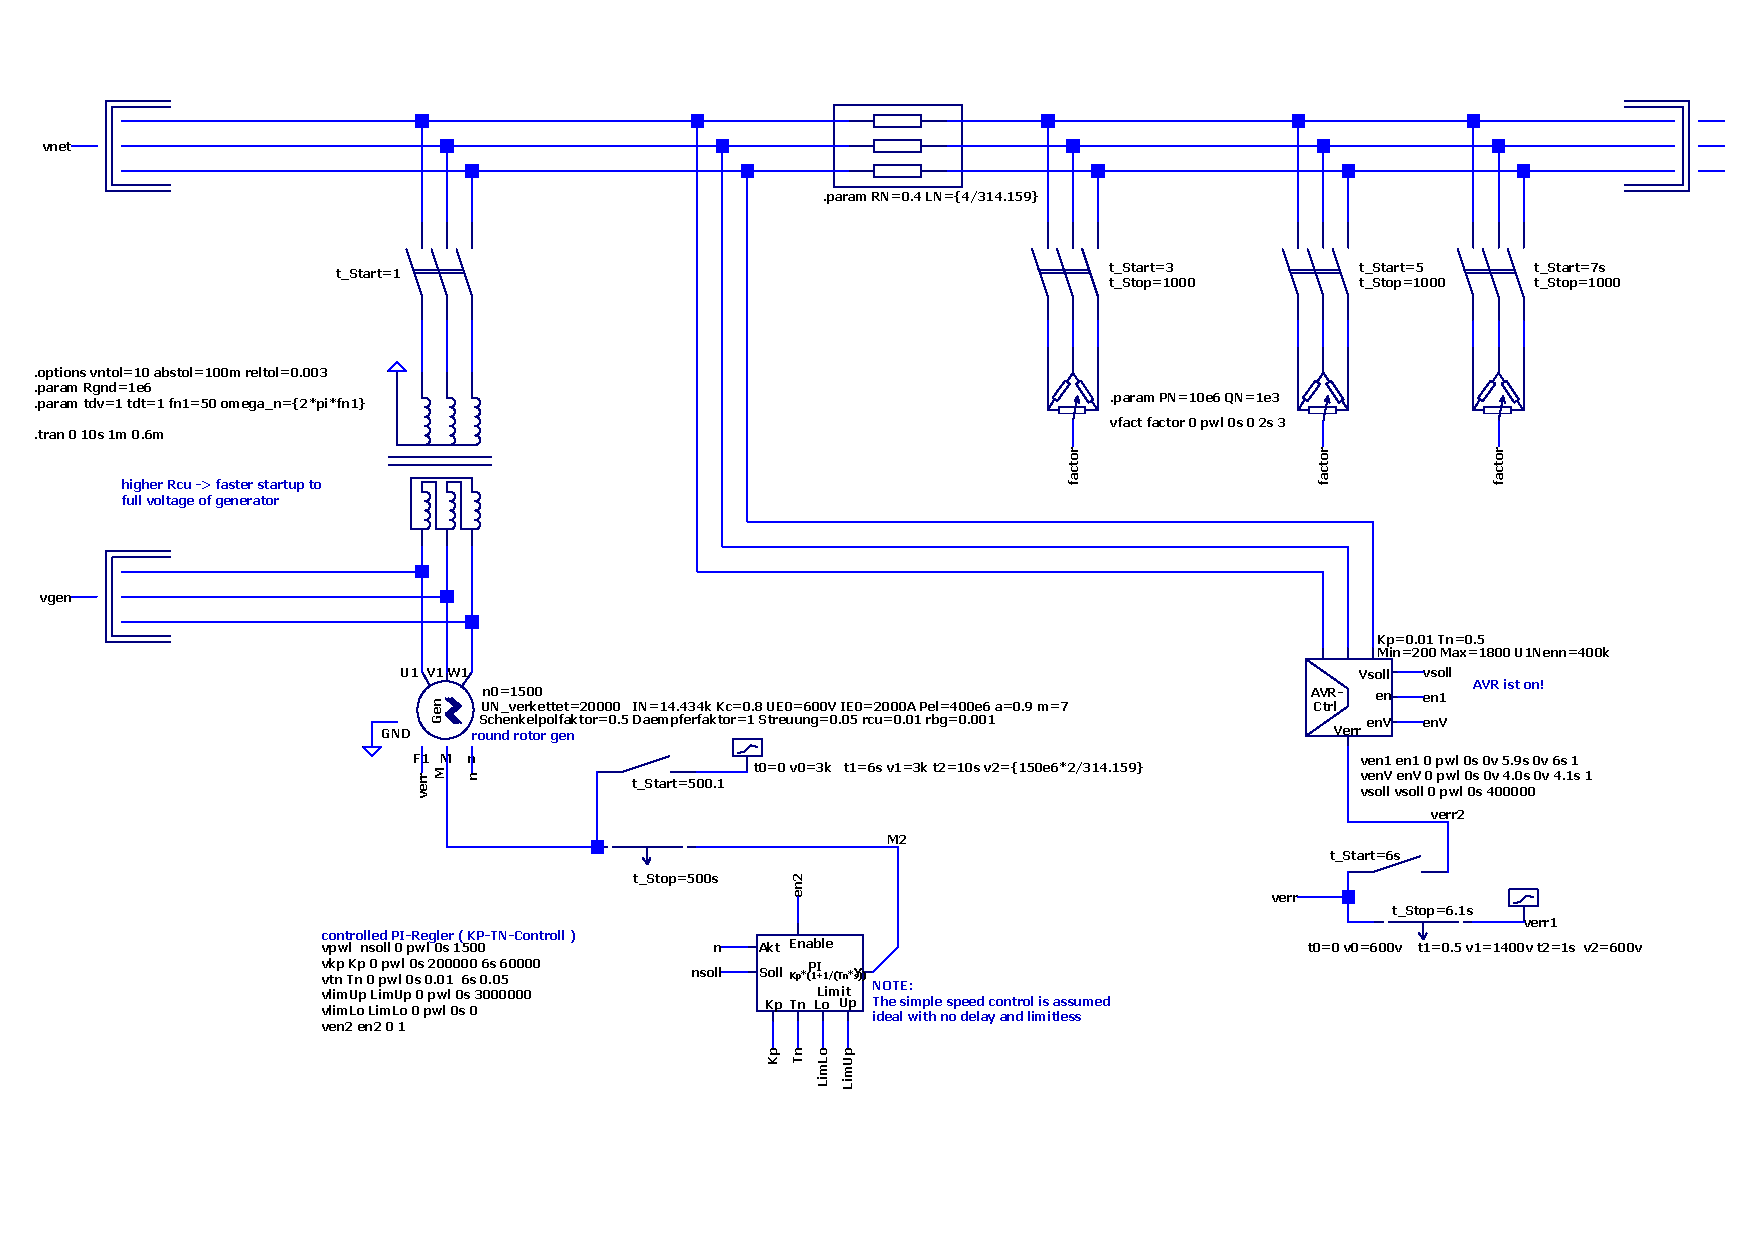
\includegraphics[width=1\textwidth] {figures/08_Synchronous_Generator/Synchronous_Generator_Isolated_mode_500MVA/Salientpole_IslandOperation_Schematic.pdf}
	\caption{Comparison with a salient-pole machine - schematic}
	\label{fig:figure87}
\end{figure}

\begin{figure}[H]
	\centering
	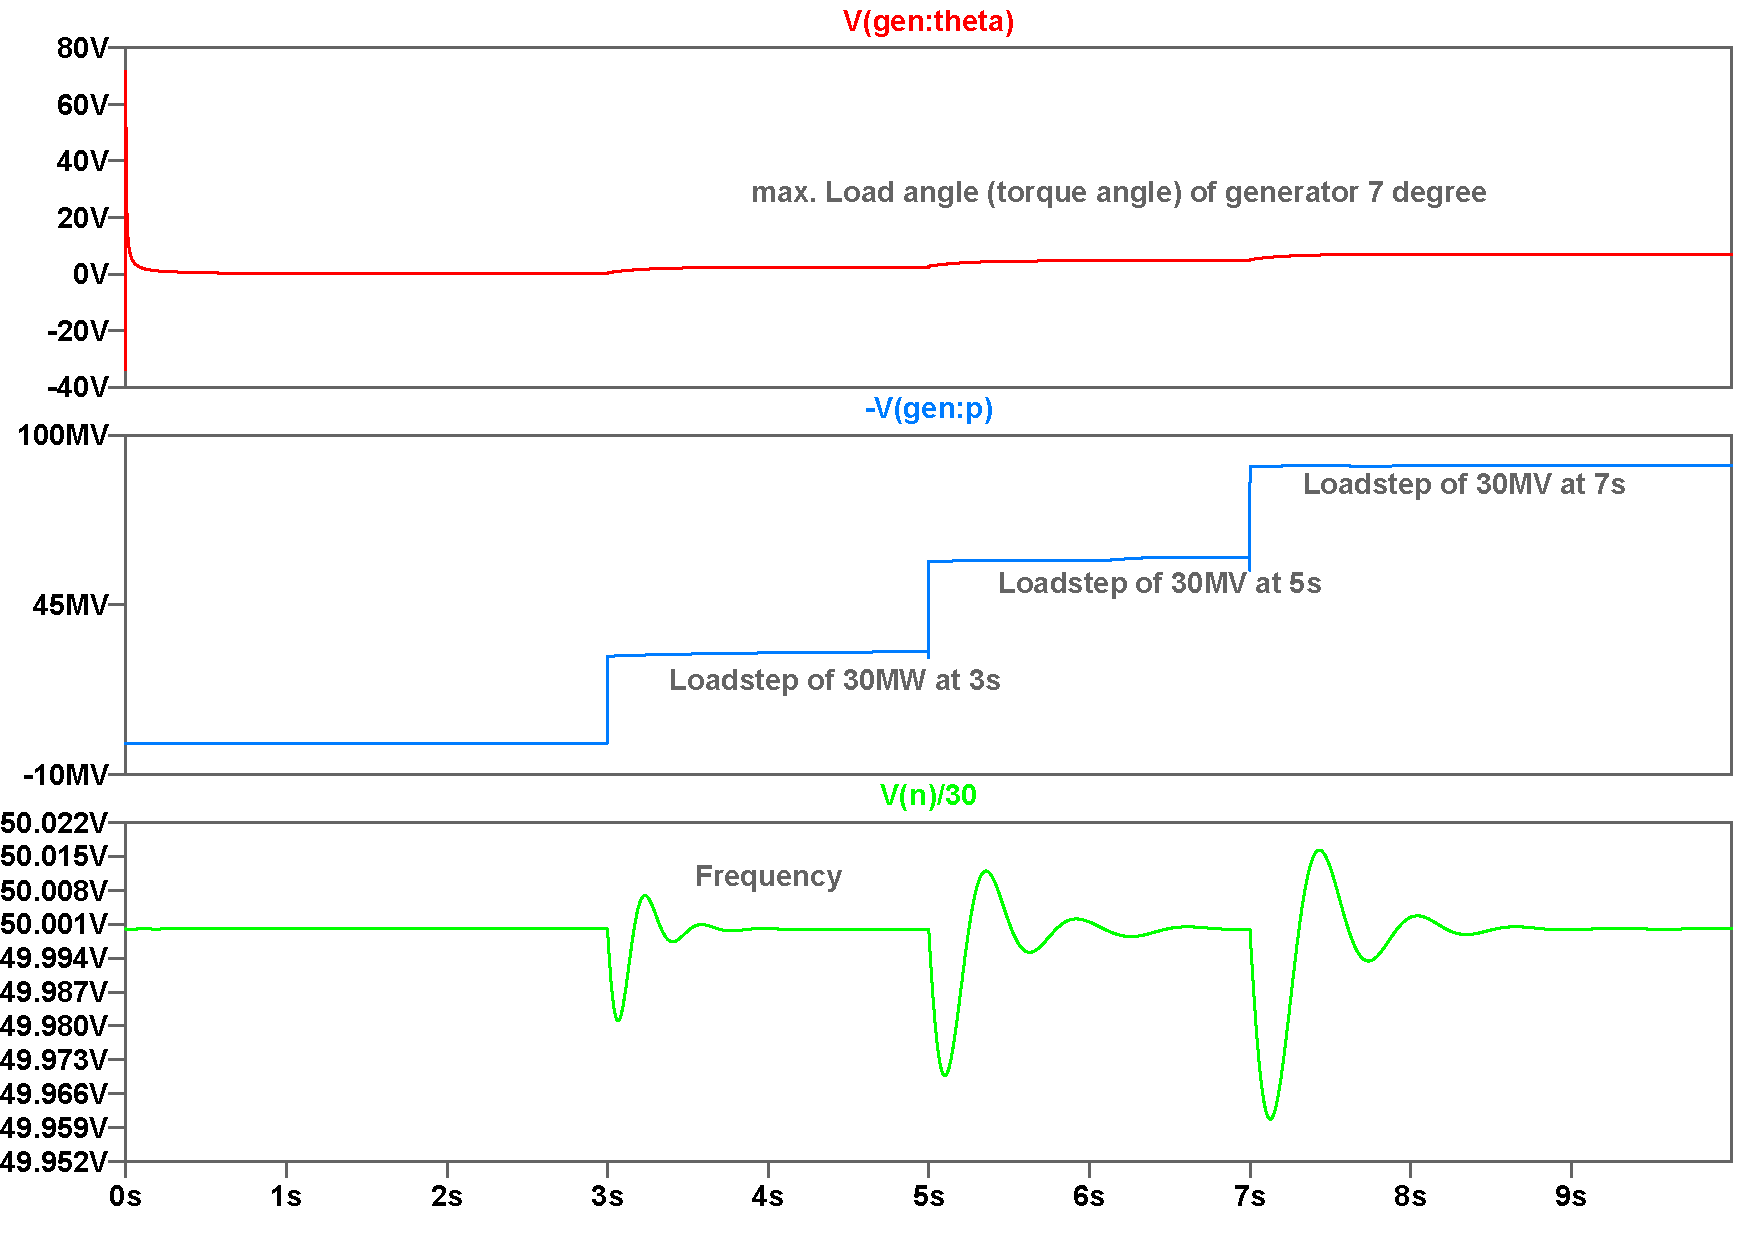
\includegraphics[width=0.9\textwidth] {figures/08_Synchronous_Generator/Synchronous_Generator_Isolated_mode_500MVA/Salientpole_IslandOperation_Waveform.pdf}
	\caption{Comparison with a salient-pole machine - Waveform}
	\label{fig:figure88}
\end{figure}

\begin{figure}[H]
	\centering
	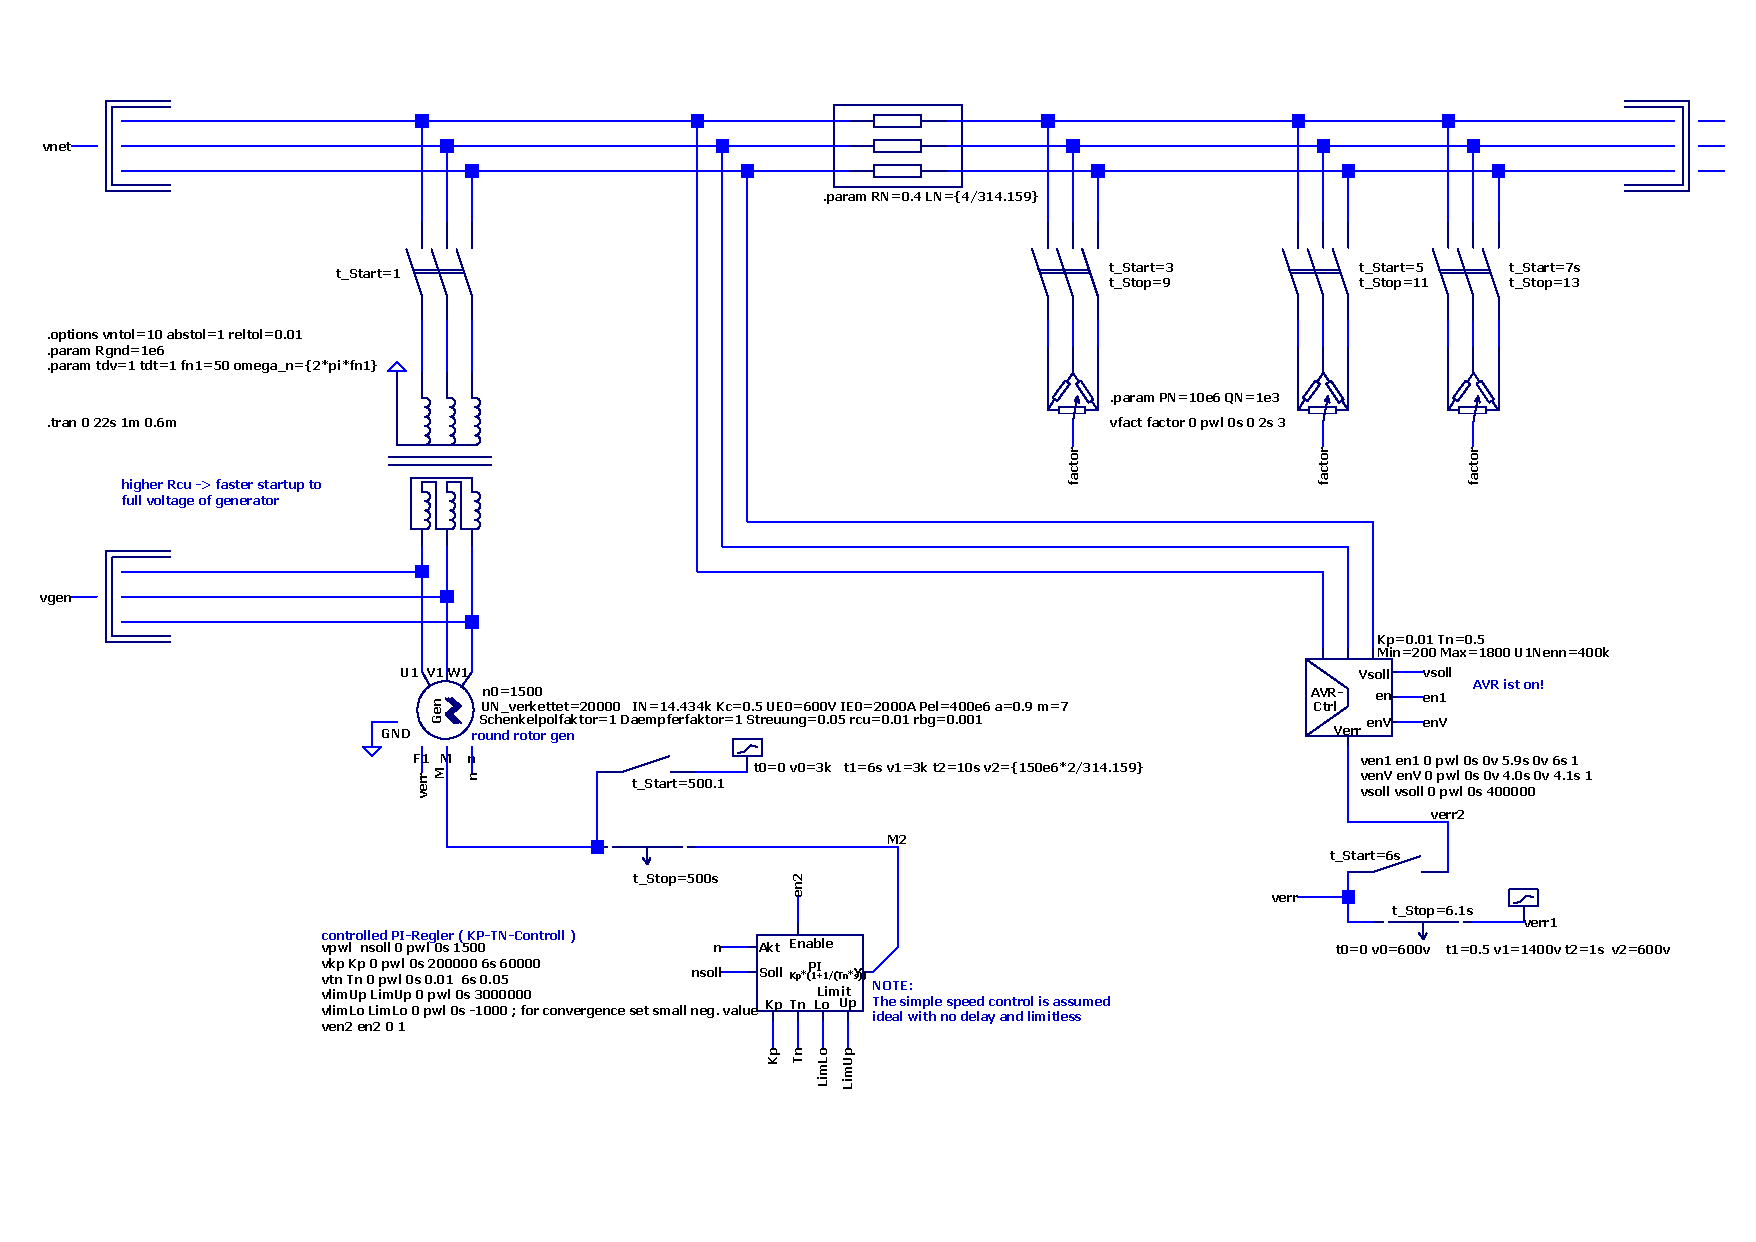
\includegraphics[width=1\textwidth] {figures/08_Synchronous_Generator/Synchronous_Generator_Isolated_mode_500MVA/Switching_off_loads_Schematic.pdf}
	\caption{Switching off loads - schematic}
	\label{fig:figure89}
\end{figure}

\begin{figure}[H]
	\centering
	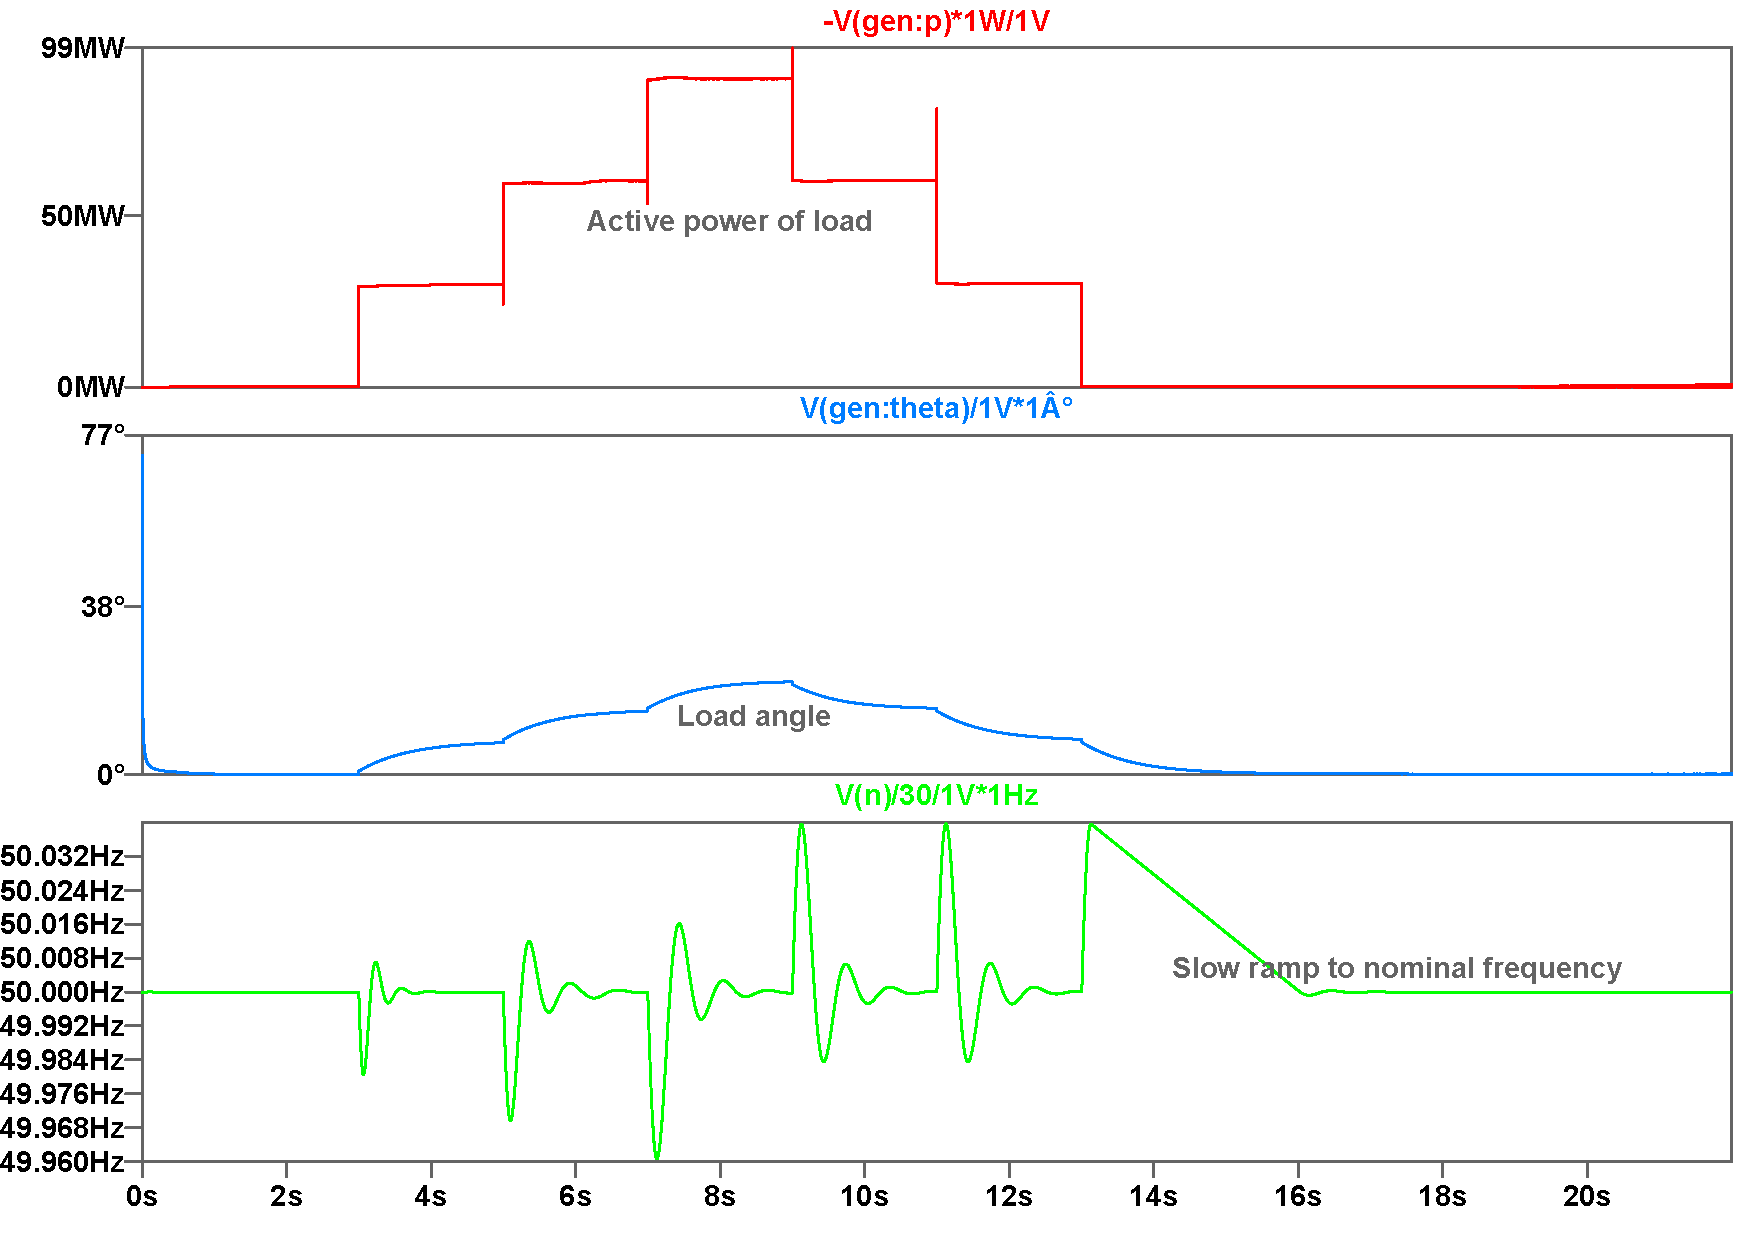
\includegraphics[width=0.9\textwidth] {figures/08_Synchronous_Generator/Synchronous_Generator_Isolated_mode_500MVA/Switching_off_loads_Waveform.pdf}
	\caption{Switching off loads - Waveform}
	\label{fig:figure810}
\end{figure}

\subsection{Synchronizing a Second Generator} see figures \ref{fig:figure811}-\ref{fig:figure813}  (simulation-file: same name as the heading)

A second generator is added on the right-hand side together with its speed
controller, but without an active AVR in this particular demonstration. The
simulation end time is increased to \SI{30}{\second}. Generator~2 is connected
at \SI{12}{\second}; its speed controller is disabled at that instant, and a
constant-torque input becomes active at \SI{12.1}{\second}. A ramp from zero
to \SI{20}{\mega\watt} between \SI{14}{\second} and
\SI{18}{\second} establishes its active-power output. A third load is switched
at \SI{20}{\second} to examine the response after synchronization.

\subsubsection{Synchronization Conditions} see figures \ref{fig:figure811} and \ref{fig:figure812} and \ref{fig:figure813}

Between approximately \SI{9.8}{\second} and \SI{10.2}{\second}, the generator
and network voltages have nearly equal magnitudes, although Generator~2 leads
slightly in phase. Its speed reference can be reduced from \SI{50}{\hertz} to
\SI{49.98}{\hertz}, corresponding to a small negative slip. At
\SI{12}{\second}, the two voltages are approximately in phase and the switch
can be closed.

\begin{important}{Conditions before synchronization}{imp:synchronization}
Before connecting a synchronous generator to an energized network, verify the
phase sequence, voltage magnitude, frequency, and phase angle. Closing the
switch with an excessive mismatch can produce high currents and severe shaft-torque transients.
\end{important}

\subsubsection{Power Sharing} see figures \ref{fig:figure811} and \ref{fig:figure812} and \ref{fig:figure813}

Generator~2 supplies \SI{20}{\mega\watt}, so Generator~1 reduces its output to
approximately \SI{40}{\mega\watt}. A subsequent
\SI{30}{\mega\watt} load step is supplied almost entirely by Generator~1,
because the active-power controller of Generator~2 has been disabled. The final
outputs are therefore approximately \SI{70}{\mega\watt} for Generator~1 and
\SI{20}{\mega\watt} for Generator~2. Generator~2 exhibits larger transient
speed deviations because it has no active governor in this example.

\begin{remark}{Regulation of parallel generators}{rem:parallel-regulation}
Disabling the AVR and governor of Generator~2 is a deliberate simplification
of this example, not a general operating rule. In practical island systems,
parallel generators normally retain coordinated voltage and speed control with
appropriate droop settings.
\end{remark}

\begin{figure}[H]
	\centering
	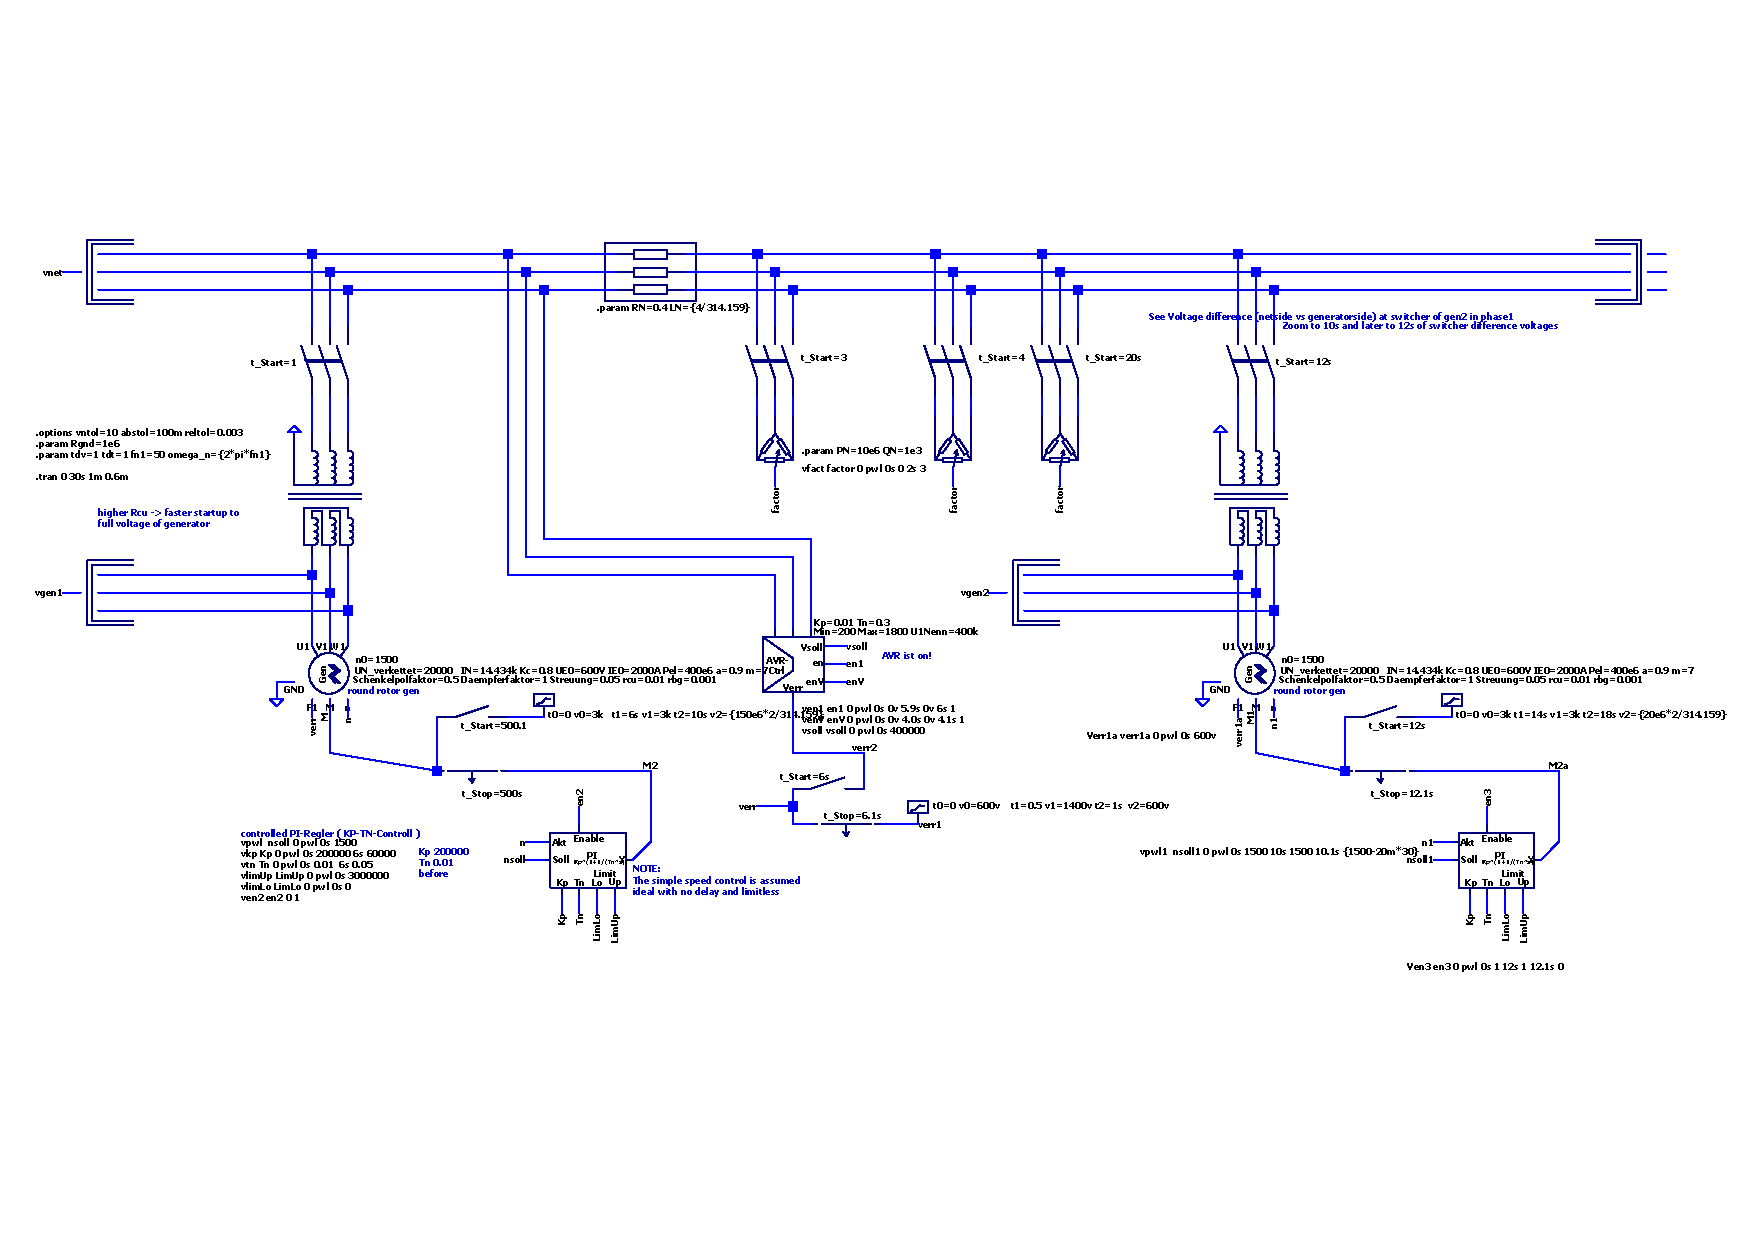
\includegraphics[width=1\textwidth] {figures/08_Synchronous_Generator/Synchronous_Generator_Isolated_mode_500MVA/Synchronizing_a_second_generator_Schematic.pdf}
	\caption{Synchronizing a second generator - schematic}
	\label{fig:figure811}
\end{figure}

\begin{figure}[H]
	\centering
	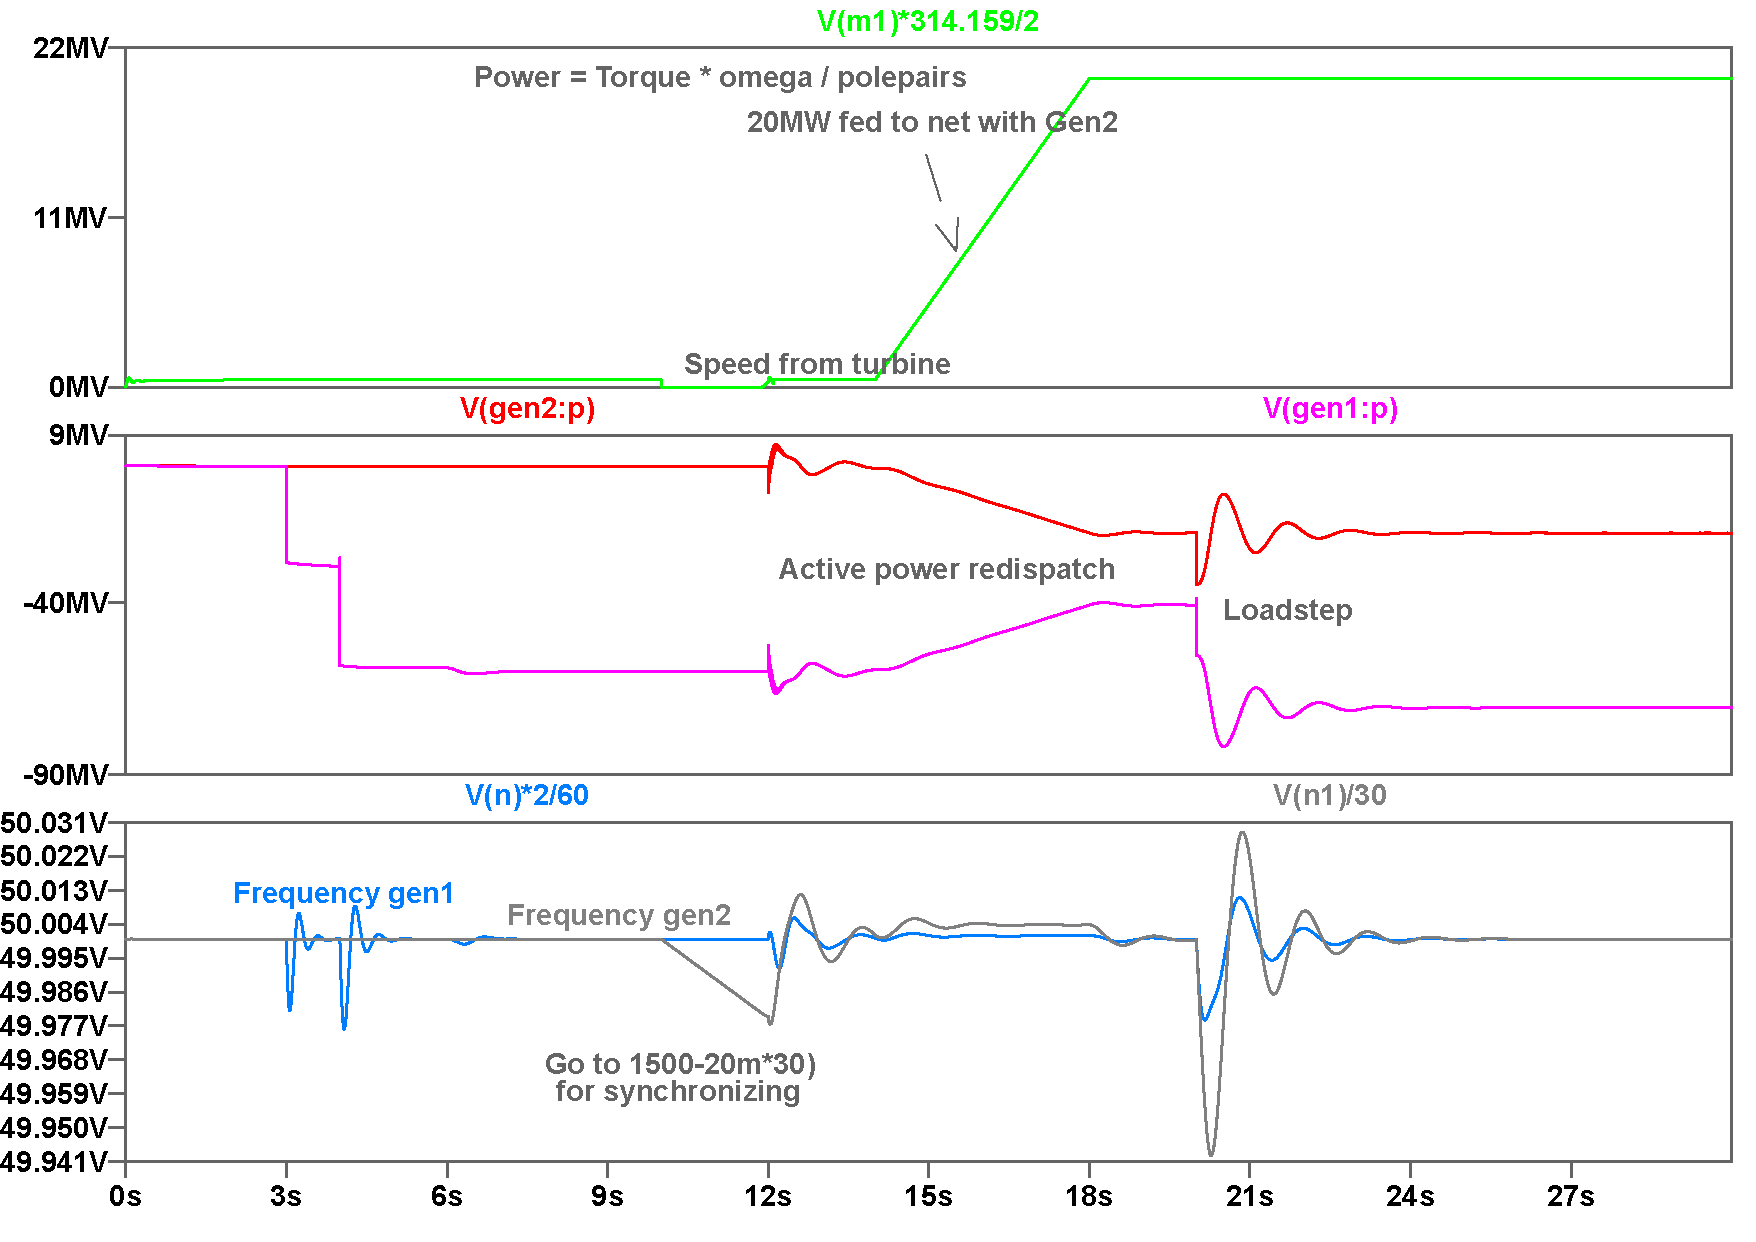
\includegraphics[width=0.9\textwidth] {figures/08_Synchronous_Generator/Synchronous_Generator_Isolated_mode_500MVA/Synchronizing_a_second_generator_Waveform.pdf}
	\caption{Synchronizing a second generator - Waveform}
	\label{fig:figure812}
\end{figure}

\begin{figure}[H]
	\centering
	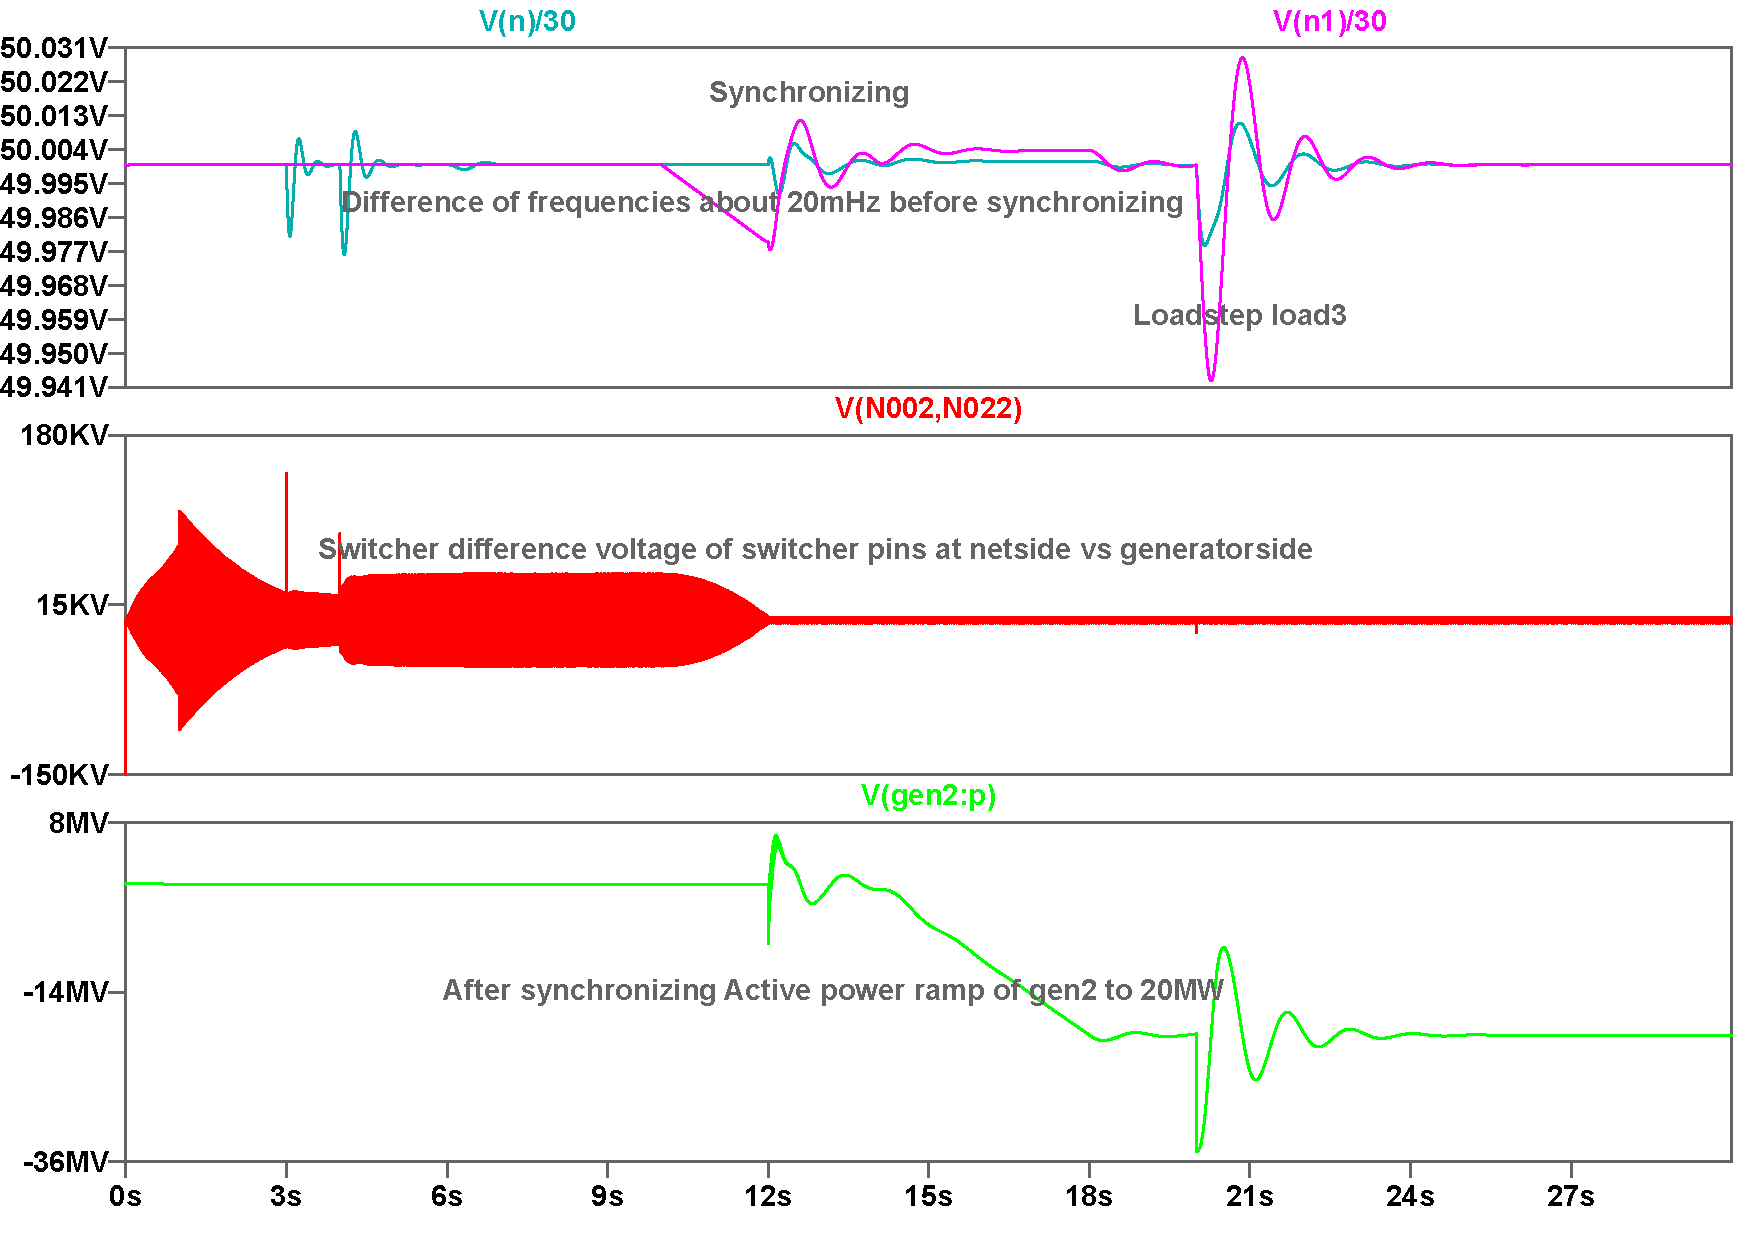
\includegraphics[width=0.9\textwidth] {figures/08_Synchronous_Generator/Synchronous_Generator_Isolated_mode_500MVA/Synchronizing_a_second_generator_Waveform2.pdf}
	\caption{Synchronizing a second generator - Waveform2}
	\label{fig:figure813}
\end{figure}


\newpage

% ============================================================
\section{Grid-Connected and Constant-Speed Operation}
\label{sec:sg-grid-and-fixed-speed}
% ============================================================

\subsection{General}

The following simulations examine synchronization with a stiff grid and the
subsequent delivery of active and reactive power. They also cover faults near
and far from the generator, a single-phase-to-ground fault, operation at fixed
speed, and the loss of synchronism when the transferable active power is
exceeded.

\subsection{Circuit Design}

From left to right, the circuit \texttt{Synchronization\_and\_active\_Power\_output.asc} contains:

\begin{itemize}
  \item a \SI{250}{\mega\volt\ampere}, \SI{13.8}{\kilo\volt},
        \SI{60}{\hertz} synchronous generator rated at
        \SI{3600}{\rpm};
  \item a speed governor and a \SI{5}{\mega\watt} auxiliary load;
  \item an AVR measuring the \SI{13.8}{\kilo\volt} generator bus;
  \item a Yd11 step-up transformer;
  \item a synchronization switch and a \SI{10}{\mega\watt} load;
  \item a switch for a three-phase-to-ground fault; and
  \item a grid impedance and a \SI{230}{\kilo\volt} stiff voltage source.
\end{itemize}

The high-voltage transformer winding is star-connected, while the
generator-side winding is delta-connected. The delta provides a path for
triplen harmonic currents. For the synchronization study, the transformer is
made linear with \texttt{M=1}; the model parameter \texttt{err0=1} is also used
to suppress nonlinear energization transients when full voltage is applied.

The rated excitation voltage is \SI{200}{\volt}. The AVR is enabled at
\SI{0.1}{\second} and provides an excitation range from
\SI{100}{\volt} to \SI{400}{\volt}, allowing both underexcited and
overexcited operation. The speed governor starts with a reference of
\SI{3600}{\rpm}.

The generator is synchronized at \SI{1}{\second}. Immediately afterwards,
the governor is disabled and the mechanical input power is ramped from zero to
\SI{150}{\mega\watt} between \SI{2}{\second} and
\SI{10}{\second}. For a machine with $p$ pole pairs,

\begin{calculation}{Mechanical power and shaft torque}{calc:sg-torque}
\begin{align}
  P_{\mathrm{m}} &= T_{\mathrm{m}}\omega_{\mathrm{m}}, \\
  \omega_{\mathrm{e}} &= p\,\omega_{\mathrm{m}}, \\
  T_{\mathrm{m}} &= \frac{pP_{\mathrm{m}}}{\omega_{\mathrm{e}}}.
\end{align}

For the two-pole turbo-generator, $p=1$ and
$\omega_{\mathrm{m}}=\omega_{\mathrm{e}}$.
\end{calculation}

To compensate the \ang{30} displacement of the Yd11 transformer during the
initial synchronization study, the grid-source phase parameter is set to
\texttt{DPHI=330}. The exact sign depends on the voltage reference directions
used in the schematic and should be confirmed from the voltage difference
across the open synchronization switch.

\subsection{Synchronization and Active-Power Output} see figures \ref{fig:figure814} and \ref{fig:figure815}   (simulation-file: same name as the heading)

In a simulation from zero to \SI{12}{\second}, the synchronization condition
at \SI{1}{\second} can be checked from the voltage difference across the open
switch. In this example, its instantaneous magnitude is approximately
\SI{4}{\kilo\volt}, and the frequencies on both sides are close to
\SI{60}{\hertz}.

Closing the switch produces transient active-power and frequency oscillations.
While the active power is being increased, the rotor speed can remain slightly
above synchronous speed. Once the input-power ramp becomes constant, the
frequency returns to \SI{60}{\hertz}. The power ramp is generated by applying
the corresponding torque ramp to the generator input pin \texttt{M-PIN}.

\begin{remark}{Accelerated simulation}{rem:active-power-ramp}
An active-power ramp of approximately \SI{19}{\mega\watt\per\second} is 
faster than would normally be used for a large generating unit. It is selected
here only to keep the simulation time short.
\end{remark}

\subsection{Three-Phase Fault in the Grid} see figures \ref{fig:figure816}-\ref{fig:figure818}  (simulation-file: same name as the heading)

A three-phase-to-ground fault is applied in the grid from
\SI{12}{\second} to \SI{12.1}{\second}. For a restarted simulation using a
saved operating point, the corresponding local time interval may appear as
\SI{0.5}{\second} to \SI{0.6}{\second}. The AVR partly supports the voltage
by increasing the excitation.

During the fault, the exported active power decreases and the load angle moves
towards zero. Because the mechanical input power initially remains unchanged,
the rotor accelerates and its kinetic energy increases until the fault is
cleared. With an end time of \SI{13}{\second} and a saved state at
\SI{11.5}{\second}, the peak fault current is approximately
\SI{58}{\kilo\ampere}; the high current persists for the
\SI{0.1}{\second} fault duration.


\begin{figure}[H]
	\centering
	\includegraphics[width=1\textwidth] {figures/08_Synchronous_Generator/Synchronous_Generator_netoperation_250MVA/Synchronization_and_active_Power_output_schematic.pdf}
	\caption{Synchronization and active power output - schematic}
	\label{fig:figure814}
\end{figure}

\begin{figure}[H]
	\centering
	\includegraphics[width=0.9\textwidth] {figures/08_Synchronous_Generator/Synchronous_Generator_netoperation_250MVA/Synchronization_and_active_Power_output_Waveform.pdf}
	\caption{Synchronization and active power output - Waveform}
	\label{fig:figure815}
\end{figure}

\begin{figure}[H]
	\centering
	\includegraphics[width=1\textwidth] {figures/08_Synchronous_Generator/Synchronous_Generator_netoperation_250MVA/Three_phase_fault_in_the_Grid_schematic.pdf}
	\caption{Three-phase fault in the grid - schematic}
	\label{fig:figure816}
\end{figure}

\begin{figure}[H]
	\centering
	\includegraphics[width=0.9\textwidth] {figures/08_Synchronous_Generator/Synchronous_Generator_netoperation_250MVA/Three_phase_fault_in_the_Grid_Waveform.pdf}
	\caption{Three-phase fault in the grid - Waveform}
	\label{fig:figure817}
\end{figure}

\begin{figure}[H]
	\centering
	\includegraphics[width=0.9\textwidth] {figures/08_Synchronous_Generator/Synchronous_Generator_netoperation_250MVA/Three_phase_fault_in_the_Grid_Waveform2.pdf}
	\caption{Three-phase fault in the grid - Waveform2}
	\label{fig:figure818}
\end{figure}

\vspace{0.2cm}
\vspace{0.1cm}

\subsection{Three-Phase Fault Near the Generator} see figures \ref{fig:figure819} and \ref{fig:figure820}  (simulation-file: same name as the heading) 

The fault is now moved directly to the generator busbar. The terminal voltage
drops more strongly, the peak current increases to approximately
\SI{80}{\kilo\ampere}, and the load angle rises beyond \ang{90} in the
reported simulation.

Although a terminal short circuit is often described as unloading the external
network, the generator can still deliver substantial electrical power into the
fault resistance and the internal machine resistances. Here, the power
dissipated in the fault path is approximately \SI{200}{\mega\watt}, about
\SI{50}{\mega\watt} greater than the applied mechanical input. The deficit is
supplied by the rotor's \emph{kinetic} energy, causing the speed to decrease.
After fault clearing, the current and speed exhibit an approximately
\SI{2}{\hertz} electromechanical oscillation before returning to their
pre-fault values.

\begin{figure}[H]
	\centering
	\includegraphics[width=1\textwidth] {figures/08_Synchronous_Generator/Synchronous_Generator_netoperation_250MVA/Three_phase_fault_near_the_generator_schematic.pdf}
	\caption{Three phase fault near the generator - Schematic}
	\label{fig:figure819}
\end{figure}

\begin{figure}[H]
	\centering
	\includegraphics[width=0.9\textwidth] {figures/08_Synchronous_Generator/Synchronous_Generator_netoperation_250MVA/Three_phase_fault_near_the_generator_waveform.pdf}
	\caption{Three phase fault near the generator - Waveform}
	\label{fig:figure820}
\end{figure}

\subsection{Uncleared Generator-Side Fault} see figures \ref{fig:figure821} and \ref{fig:figure822}  (simulation-file: same name as the heading) 

For this study, the generator is initially operated without an external load;
only the small friction-torque input remains. Setting the fault switch
parameter \texttt{Tstop} to \SI{100}{\second} keeps the fault closed throughout
the relevant simulation interval.

The calculated electrical power initially rises to approximately
\SI{450}{\mega\watt}, producing strong braking torque. The rotor angle
decreases, crosses zero after approximately \SI{750}{\milli\second}, and
continues towards \ang{-180}. The machine then loses synchronism and passes
periodically between generating and motoring operation. Rotor acceleration,
deceleration, power reversal, and pole slipping repeat as long as the fault and
the stiff grid remain connected.

\begin{warningbox}[Unstable operating condition]
An uncleared generator-side short circuit leads to extreme electrical and
mechanical stress and loss of synchronism. Real protection systems must clear
such a fault rapidly and isolate the affected unit.
\end{warningbox}


\begin{figure}[H]
	\centering
	\includegraphics[width=1\textwidth] {figures/08_Synchronous_Generator/Synchronous_Generator_netoperation_250MVA/Uncleared_generatorside_Fault_schematic.pdf}
	\caption{Uncleared Generator-side Fault - Schematic}
	\label{fig:figure821}
\end{figure}

\begin{figure}[H]
	\centering
	\includegraphics[width=0.9\textwidth] {figures/08_Synchronous_Generator/Synchronous_Generator_netoperation_250MVA/Uncleared_generatorside_Fault_waveform.pdf}
	\caption{Uncleared Generator-side Fault - Waveform}
	\label{fig:figure822}
\end{figure}

\vspace{0.3cm}


\subsection{Generator-Side Fault at Constant Speed} see figures \ref{fig:figure823} and \ref{fig:figure824}  (simulation-file: same name as the heading)

When the generator is constrained to constant speed, the calculated peak
short-circuit current rises to approximately \SI{95}{\kilo\ampere}. The
instantaneous electromagnetic torque, expressed as an equivalent power at the
fixed speed, exceeds \SI{900}{\mega\watt} at fault inception.

The current waveform shows the short subtransient interval, followed by the
longer transient interval and finally the steady-state short-circuit current.
Although the applied excitation voltage remains constant, transformer action
between the stator and rotor circuits causes the field current to rise to about
\SI{4.4}{\kilo\ampere} before it decays towards its nominal value of
approximately \SI{200}{\ampere}. The generator terminal voltage approaches
zero, and the calculated load angle is approximately \ang{90}.


\begin{figure}[H]
	\centering
	\includegraphics[width=1\textwidth] {figures/08_Synchronous_Generator/Synchronous_Generator_netoperation_250MVA/Generatorside_Fault_at_Constant_Speed_Schematic}
	\caption{Generator-side fault at constant speed - Schematic}
	\label{fig:figure823}
\end{figure}

\begin{figure}[H]
	\centering
	\includegraphics[width=0.9\textwidth] {figures/08_Synchronous_Generator/Synchronous_Generator_netoperation_250MVA/Generatorside_Fault_at_Constant_Speed_waveform.pdf}
	\caption{Generator-side fault at constant speed - Waveform}
	\label{fig:figure824}
\end{figure}


\subsection{Single-Phase-to-Ground Fault Near the Generator} see figures \ref{fig:figure825} and \ref{fig:figure826}  (simulation-file: same name as the heading) 

For the single-phase-to-ground fault, the generator neutral point is grounded.
The simulated peak fault current is approximately \SI{110}{\kilo\ampere},
which is higher than the three-phase peak in this particular network and
grounding configuration.

Whereas the principal transients of the three-phase fault decay within about
\SI{100}{\milli\second}, the asymmetrical ground fault continues to excite
negative-sequence components. The system can be decomposed into positive-sequence (+omega) and negative-sequence (-omega) components. The negative system
rotates in the opposite direction to the rotor and induces voltages at twice the fundamental frequency in the field and damper windings. These fields can now also be divided into two rotating fields. One rotates at +omega and the other at −omega. The field with +omega compensates for the stator field, and the field with -omega now has 3*omega relative 
to the stator and induces voltages there at triple the frequency. This continues to repeat, but only the
fields with 2x to 4x the frequency are significant.

An FFT evaluated between approximately \SI{600}{\milli\second} and
\SI{800}{\milli\second} shows components at \SI{60}{\hertz},
\SI{120}{\hertz}, and \SI{240}{\hertz} in the excitation current. The stator
current contains prominent components at \SI{60}{\hertz} and
\SI{180}{\hertz}. Similar effects can occur, with smaller magnitudes, when a
synchronous generator supplies an asymmetrical load.

\vspace{10pt}

\begin{remark}{Interpretation of FFT components}{rem:sg-fft-components}
The exact harmonic spectrum depends on the machine model, saturation,
reference-frame definitions, fault inception angle, grounding impedance, and
the selected FFT window. The listed frequency components are results of this
simulation and should not be interpreted as universal amplitudes for every
synchronous machine.
\end{remark}


\begin{figure}[H]
	\centering
	\includegraphics[width=1\textwidth] {figures/08_Synchronous_Generator/Synchronous_Generator_netoperation_250MVA/Single_Phase_to_ground_fault_near_the_generator_schematic.pdf}
	\caption{Single-phase to ground fault near the generator - Schematic}
	\label{fig:figure825}
\end{figure}

\begin{figure}[H]
	\centering
	\includegraphics[width=0.9\textwidth] {figures/08_Synchronous_Generator/Synchronous_Generator_netoperation_250MVA/Single_Phase_to_ground_fault_near_the_generator_waveform.pdf}
	\caption{Single-phase to ground fault near the generator - Waveform}
	\label{fig:figure826}
\end{figure}

\begin{figure}[H]
	\centering
	\includegraphics[width=0.9\textwidth] {figures/08_Synchronous_Generator/Synchronous_Generator_netoperation_250MVA/Single_phase_to_ground_fault_near_the_generator_waveform_FFT.pdf}
	\caption{Single-phase to ground fault near the generator - Waveform}
	\label{fig:figure827}
\end{figure}



\subsection{Phasor Diagram During a Continuous Fault} see figures \ref{fig:figure828}-\ref{fig:figure833}  (simulation-file: same name as the heading) 

For a steady-state phasor diagram at constant speed, read the values
\texttt{Usx}, \texttt{Usy}, \texttt{Isx}, \texttt{Isy}, \texttt{Imx}, and \texttt{Imy} from  the LTspice
waveform viewer at \SI{8.5}{\second}. Enter these quantities in the wxMaxima file
\begin{center}
\texttt{synchrongenerator.wxmx}
\end{center}
The script scales the values and calculates the additional quantities required
by the phasor diagram. The values of $X_d$ and $X_q$ are taken from
%\begin{center}
\texttt{synchrongeneratordata.wxmx}.
%\end{center}
Finally, transfer the calculated vectors to the GeoGebra file
%\begin{center}
\texttt{synchrongenerator.ggb}.
%\end{center}

Because \texttt{Usx} and \texttt{Usy} are very small, their vector sum, the
terminal voltage $\vect{U}$, is almost zero. The internal excitation voltage is
large and lies on the quadrature axis. The stator current lies approximately on
the negative real axis, whereas the small terminal voltage lies on the positive
real axis. Under the sign convention used here, the machine therefore delivers
mainly active power into the resistive fault path. The corresponding loss is
approximately \SI{2}{\mega\watt}. 

For a subtransient phasor diagram shortly
after fault inception, zoom into the interval from \SI{500}{\milli\second} to
\SI{520}{\milli\second} and read the values at approximately
\SI{515.95}{\milli\second}. In addition to the stator quantities, record the
damper-current components \texttt{IDx} and \texttt{IDy}. Scale these values in
\begin{center}
\texttt{synchrongeneratorwithdamper.wxmx}
\end{center}
before transferring them to GeoGebra. The resulting diagram shows the strong
initial influence of the damper winding. 
NOTE: The Phasor diagram uses the load reference arrow system convention.

\begin{figure}[H]
	\centering
	\includegraphics[width=1\textwidth] {figures/08_Synchronous_Generator/Synchronous_Generator_netoperation_250MVA/Phasor_Diagramm_During_a_continuous_Fault_schematic.pdf}
	\caption{Phasor diagram during a sustained fault - Schematic}
	\label{fig:figure828}
\end{figure}

\begin{figure}[H]
	\centering
	\includegraphics[width=0.9\textwidth] {figures/08_Synchronous_Generator/Synchronous_Generator_netoperation_250MVA/Phasor_Diagramm_During_a_continuous_Fault_waveform.pdf}
	\caption{Phasor diagram during a sustained fault - Waveform}
	\label{fig:figure829}
\end{figure}

\begin{figure}[H]
	\centering
	\includegraphics[width=0.9\textwidth] {figures/08_Synchronous_Generator/Synchronous_Generator_netoperation_250MVA/Phasor_Diagramm_During_a_continuous_Fault_with_damper_schematic.pdf}
	\caption{Phasor diagram during a sustained fault with damper - Schematic}
	\label{fig:figure830}
\end{figure}

\begin{figure}[H]
	\centering
	\includegraphics[width=0.9\textwidth] {figures/08_Synchronous_Generator/Synchronous_Generator_netoperation_250MVA/Phasor_Diagramm_During_a_continuous_Fault_with_damper_waveform.pdf}
	\caption{Phasor diagram during a sustained fault with damper - Waveform}
	\label{fig:figure831}
\end{figure}

\begin{figure}[H]
	\centering
	\includegraphics[width=0.9\textwidth] {figures/08_Synchronous_Generator/Synchronous_Generator_netoperation_250MVA/Synchrongenerator_with_damper.png}
	\caption{Phasor Diagramm without damper subtransient - Waveform}
	\label{fig:figure832}
\end{figure}

\begin{figure}[H]
	\centering
	\includegraphics[width=0.9\textwidth] {figures/08_Synchronous_Generator/Synchronous_Generator_netoperation_250MVA/Synchrongenerator.jpg}
	\caption{Phasor Diagramm with damper steady state - Waveform}
	\label{fig:figure833}
\end{figure}


\subsection{Active- and Reactive-Power Control}  see figures \ref{fig:figure834}-\ref{fig:figure837}  (simulation-file: same name as the heading) 

Active power is controlled through the mechanical torque applied at the
generator's \texttt{M} input. The speed governor must first be changed from
speed-regulating operation to the intended grid-connected power-control mode.
In the example, the machine is ramped to \SI{100}{\mega\watt}, during which the
load angle rises to approximately \ang{10}. The fault switch is disabled by
placing its stop time outside the simulated interval.

Reactive power is varied by changing the field supply at \texttt{Verr} from
\SI{200}{\volt} to \SI{100}{\volt} between \SI{11}{\second} and
\SI{13}{\second}, and then from \SI{100}{\volt} to \SI{400}{\volt} between
\SI{13}{\second} and \SI{15}{\second}. Increasing the excitation reduces the
load angle for the chosen active power and improves the steady-state stability
margin. Because the stiff grid largely fixes the terminal voltage, excitation
mainly changes reactive power. This differs from island operation, where
excitation has a much stronger influence on voltage.

For a deliberately fast demonstration, the field-resistance parameter can be
set to \texttt{RE=1e4}. At \SI{200}{\volt}, the reactive-power exchange is
approximately zero. Reducing the excitation to \SI{100}{\volt} makes the
underexcited generator absorb reactive power; increasing it to
\SI{400}{\volt} makes the overexcited generator supply reactive power.

\begin{remark}{Artificial field resistance}{rem:artificial-field-resistance}
Changing \texttt{RE} to accelerate the response is useful for demonstrating
the qualitative relationship between excitation and reactive power, but it no
longer represents the original physical field time constant.
\end{remark}

\begin{figure}[H]
	\centering
	\includegraphics[width=0.9\textwidth] {figures/08_Synchronous_Generator/Synchronous_Generator_netoperation_250MVA/Active_and_reactive_power_control_schematic.pdf}
	\caption{Active and reactive power control - Schematic}
	\label{fig:figure834}
\end{figure}

\begin{figure}[H]
	\centering
	\includegraphics[width=0.9\textwidth] {figures/08_Synchronous_Generator/Synchronous_Generator_netoperation_250MVA/Active_and_reactive_power_control_waveform.pdf}
	\caption{Active and reactive power control - Waveform}
	\label{fig:figure835}
\end{figure}

\begin{figure}[H]
	\centering
	\includegraphics[width=0.9\textwidth] {figures/08_Synchronous_Generator/Synchronous_Generator_netoperation_250MVA/Active_and_reactive_power_control2_schematic.pdf}
	\caption{Active and reactive power control zoomed - Schematic}
	\label{fig:figure836}
\end{figure}

\begin{figure}[H]
	\centering
	\includegraphics[width=0.9\textwidth] {figures/08_Synchronous_Generator/Synchronous_Generator_netoperation_250MVA/Active_and_reactive_power_control2_waveform.pdf}
	\caption{Active and reactive power control zoomed - Waveform}
	\label{fig:figure837}
\end{figure}


\subsection{Phasor Diagrams for Overexcited and Underexcited Operation}  see figures \ref{fig:figure838}-\ref{fig:figure840}  (simulation-file: same name as the heading) 

An overexcited synchronous generator operates with a field current higher than the value required for approximately unity power factor. The stronger rotor magnetic field causes the generator to supply reactive power to the electrical network. Its stator current is typically lagging with respect to the terminal voltage. Overexcited generators therefore support the grid voltage and can be used for voltage regulation and reactive-power compensation.
An underexcited synchronous generator operates with a reduced field current. In this condition, the generator absorbs reactive power from the network. The stator current is typically leading with respect to the terminal voltage. Underexcited operation can therefore be used to reduce excessive grid voltage.
For a generator delivering approximately constant active power, changing the excitation mainly changes its reactive power and power factor:

\begin{itemize}
	\item Overexcited: supplies reactive power → lagging power factor,
	\item Underexcited: absorbs reactive power, and
	\item Normal excitation: reactive power is approximately zero → power factor close to unity
\end{itemize}

\begin{figure}[H]
	\centering
	\includegraphics[width=0.9\textwidth] {figures/08_Synchronous_Generator/Synchronous_Generator_netoperation_250MVA/Phasor_Diagramm_under-and-overexcited_schematic.pdf}
	\caption{synchronous generator underexcited/overexcited  - schematic}
	\label{fig:figure838}
\end{figure}

\begin{figure}[H]
	\centering
	\includegraphics[width=0.9\textwidth] {figures/08_Synchronous_Generator/Synchronous_Generator_netoperation_250MVA/Underexcitation.pdf}
	\caption{synchronous generator underexcited (plotted with GeoGebra) - phasor diagramm}
	\label{fig:figure839}
\end{figure}


\begin{figure}[H]
	\centering
	\includegraphics[width=0.9\textwidth] {figures/08_Synchronous_Generator/Synchronous_Generator_netoperation_250MVA/Overexcitation.pdf}
	\caption{synchronous generator overexcited (plotted with GeoGebra)  - phasor diagramm}
	\label{fig:figure840}
\end{figure}


\subsection{Maximum Transferable Active Power}  see figures \ref{fig:figure841}-\ref{fig:figure842}  (simulation-file: same name as the heading) 

If the mechanical input power is increased continuously, or if excitation is
reduced excessively, the load angle rises towards the static stability limit.
Its exact location depends on the machine type, excitation, network impedance,
and saliency. A round-rotor approximation has its theoretical maximum near
\ang{90}; the reluctance-torque term of a salient-pole machine changes the
power-angle characteristic and can shift this maximum.

For secure operation, a substantial angular margin must be maintained. In this
example, the load angle should remain below approximately \ang{60}. If the
stable operating range is exceeded, the rotor slips poles, active power
oscillates, and the terminal voltage can collapse severely.

\begin{warningbox}[Loss of synchronism]
Operation near or beyond the maximum of the power-angle characteristic must be
avoided. The simulation is intended to demonstrate instability, not an
allowable continuous operating condition.
\end{warningbox}


\begin{figure}[H]
	\centering
	\includegraphics[width=0.9\textwidth] {figures/08_Synchronous_Generator/Synchronous_Generator_netoperation_250MVA/Maximum Transferable Active Power_schematic.pdf}
	\caption{Maximum Transferable Active Power - Schematic}
	\label{fig:figure841}
\end{figure}

\begin{figure}[H]
	\centering
	\includegraphics[width=0.9\textwidth] {figures/08_Synchronous_Generator/Synchronous_Generator_netoperation_250MVA/Maximum Transferable Active Power_waveform.pdf}
	\caption{Maximum Transferable Active Power - Waveform}
	\label{fig:figure842}
\end{figure}

\begin{chaptersummary}
In island operation, voltage and frequency must be established by the
generating units. The AVR regulates voltage, while the governor balances
mechanical power and load demand. Parallel island generators require
coordinated control and careful synchronization.

When connected to a stiff grid, mechanical torque mainly controls active
power, whereas excitation mainly controls reactive power. Fault location,
fault symmetry, grounding, rotor dynamics, and the selected mechanical-speed
model strongly influence the short-circuit current and electromechanical
response. Excessive load angle leads to loss of synchronism and must be
prevented by suitable operating limits and protection.
\end{chaptersummary}
